\begin{figure}[H]%
	\ThisCenterWallPaper{1}{images/\texorpdfstring{\chaptername\thechapter}}%
	\captionlistentry[figure]{Icon of \chaptername\ \thechapter}% figure with chapter and section number
	%\addcontentsline{lof}{figure}{Icon of \chaptername\ \thechapter}% figure without chapter and section number
	\label{fig:\chaptername\thechapter}%
\end{figure}%

\vspace*{-6.4cm}
\epigraph{"In the digital universe, our personal history and its sense of narrative is succeeded by our social networking profile - a snapshot of the current moment. The information itself - our social graph of friends and likes - is a product being sold to market researchers in order to better predict and guide our futures."}{\textit{--- Douglas Rushkoff}}

\noindent \large{\textbf{This {\MakeLowercase{\chaptername}}'s contents:}}
\vspace*{-0.75cm}
\minitoc \mtcskip \minilof
\vspace*{-0.5cm}
\section{The hardware and the OS} \label{section:ImplementingtheWebApp/ThehardwareandtheOS}
In order to host the application with all its components, different machines were bought.
These include 5 general purpose used computers, 1 programmable new router, a new network switch (after the first one stopped working during the development phase), 2 used monitors and lots of cables.

\subsection{The machines} \label{subsection:ImplementingtheWebApp/Thehardware/Themachines}
The bought computers were 2 Lenovo ThinkCentre M73 Tiny Form Factor - each with 8 GB of RAM, CPU Intel Core i3-4130 4 cores, 3.4GHz and an SSD harddrive of 250 GB.
Apart from the Lenovo-s, 2 HP Compaq 8200 Elite Small Farm Factor were bought - each with 8 GB of RAM, CPU Intel Core i5-2400, 4 cores, 3.1 GHz and an SSD of 120 GB.
Another last machine with similar specifications was bought but was never used because it was decided to put the database in a single machine, thus not creating a cluster.
A photo of the machines is diplayed in \hyperref[fig:machinesphoto]{\autoref{fig:machinesphoto}}.

\begin{figure}[H]%
	\centering%
	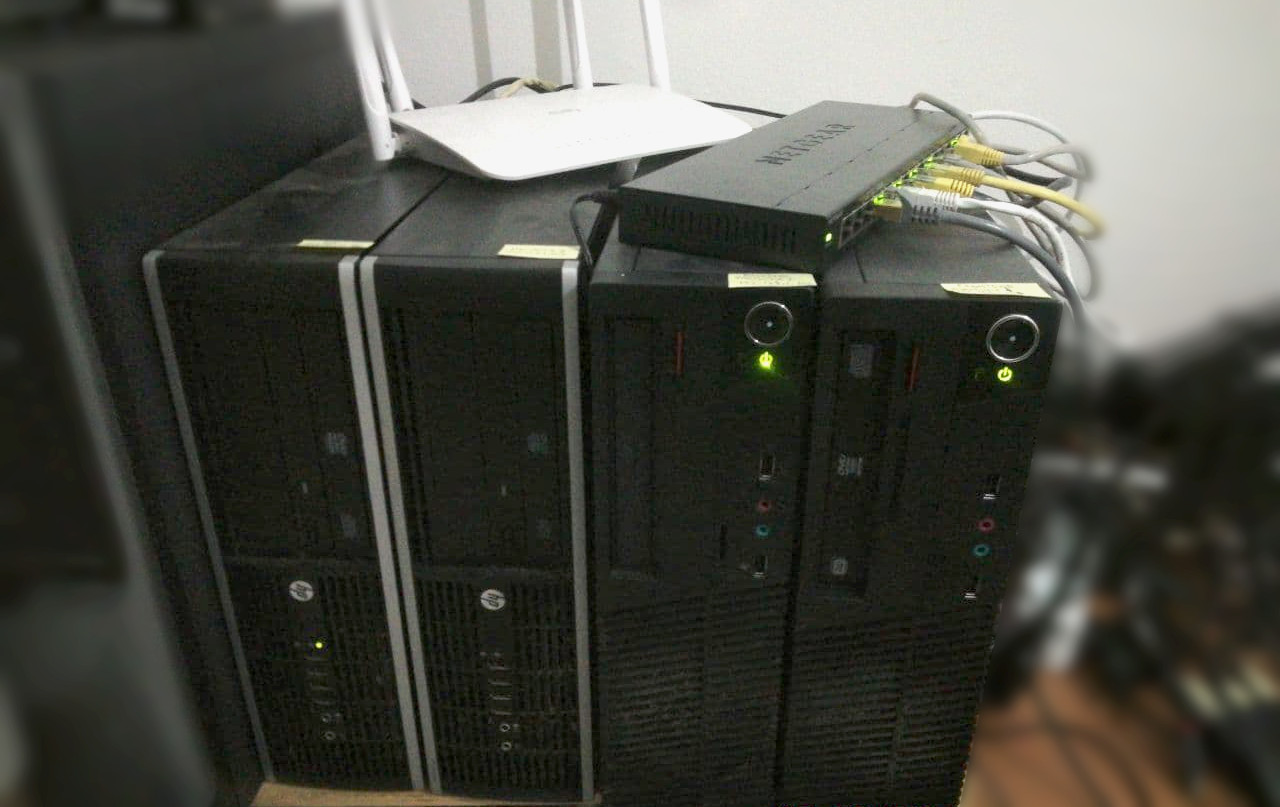
\includegraphics[%
		width=1\textwidth-4pt,%
		bgcolor=white,%
		cfbox=lightestgray % color
			  2pt % rule width
			  0pt % rule separation
			  0pt % margin
	]{images/chapter4/machinesphoto.jpg}%
	\caption[Photo of the computers, router and switch used for hosting the Web App \acrshort{API}, frontend UI and the database]{Photo of the computers, router and switch used for hosting the Web App \acrshort{API}, frontend UI and the database}%
	\label{fig:machinesphoto}
\end{figure}%

One machine is being used as a server for the frontend.
A second machine is being used as a server of the \acrshort{API}, the backend.
A third machine hosts the database, an ArangoDB on single node.
The fourth machine is used for development, deployment and remote access purposes.

\subsection{The network} \label{subsection:ImplementingtheWebApp/Thehardware/Thenetwork}
The network is setup in a home environment.
The CUDY WR1300 router of MediaTek MT7621 architecture routes the connection from the main (and distant) home router to the network switch.
The CUDY router is connected in client (bridge) mode to the main home router.
Before setting up the network, CUDY's firmware was changed from the stock one to a new version and than to OpenWRT 19.07. This was made to have full control of the configurations of the router.

The switch, a NETGEAR Switch Ethernet Gigabit GS316, switches the connection from CUDY to all the machines.

\subsection{Setup} \label{subsection:ImplementingtheWebApp/Thehardware/Setup}
In the home router some configurations are made to expose CUDY directly to the Internet.
In CUDY static IP addresses and symbolic hostnames are assigned to DHCP clients (the computers).
In the routers firewall port forwarding is setup to allow access to the server of the frontend of the website.
Also a Dynamic DNS service is setup to help with the dynamic IP changes.

On the computers \gls{CentOS} Linux 7 (Core) is installed, kernel version: \texttt{Linux 3.10.0-1160.el7.x86\_64}.
On the \gls{frontend server} the usual configurations for serving a website are made.
On the \gls{backend server} Nodejs and \texttt{pm2} is installed.
On the DB host ArangoDB is installed.

ArangoDB GDBMS is installed on one of the machines.

A dummy application is deployed on the machines - some example data is imported on an ArangoDB collection, a ready-made Rest \acrshort{API} is setup on the \gls{backend server} and a frontend interface is placed in the \gls{frontend server}. A simple test visit from local network and from external network (using mobile data connection tethering) is done to the website's dyndns provided domain address. Then, on the dummy application's frontend some DB communication via \acrshort{API} requiring actions are undertaken to see if everything is working as should between the machines, the \acrshort{API} and the DB.
Having everything setup, working and briefly tested, the environment is ready to host and serve.

\section{The data} \label{section:ImplementingtheWebApp/Thedata}
\begin{figure}[H]%
	\centering%
	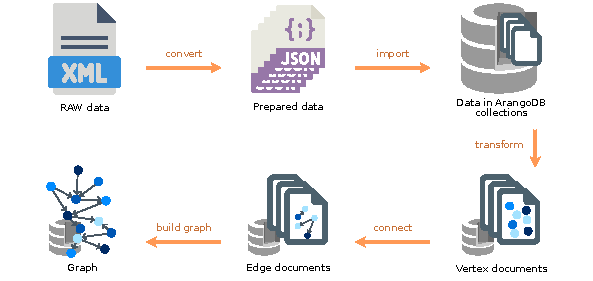
\includegraphics[width=1\textwidth,%
	]{images/chapter4/datatransformations.pdf}%
	\caption[The process of transformations of the data from dblp downloading to graph building in ArangoDB DBMS]{The process of transformations of the data from \gls{dblp.org}\sfcite{Dagstuhl2021} downloading to graph building in ArangoDB DBMS}%
	\label{fig:datatransformations}%
\end{figure}%

In this section are described all the steps carried from download of the data, their conversion, import in the database and reorganizing into vertices and edges afterwards. In the end the graph is built. See \hyperref[fig:datatransformations]{\autoref{fig:datatransformations}} for a graphical representation of the process.

In the following subsection \gls{dblp.org}\sfcite{Dagstuhl2021} dataset download and data conversion is presented.

\subsection[dblp.org dataset download and data conversion]{\gls{dblp.org}\sfcite{Dagstuhl2021} dataset download and data conversion} \label{subsection:ImplementingtheWebApp/Thedata/dblpcomdatasetdownloadanddataconversion}
As mentioned a few times now, the dataset is downloaded from \gls{dblp.org}\sfcite{Dagstuhl2021} or more precisely from \url{dblp.uni-trier.de}\sfcite{Dagstuhl2021}

The data, version of 2021-07-01 is a single .gz compressed archive of size 611MB.
Once extracted, the output is a single XML file \textit{dblp.xml} of 3.2GB in size.
From the website is possible to download also some text files on changes, README snd documentation.

\begin{figure}[H]%
	\centering%
	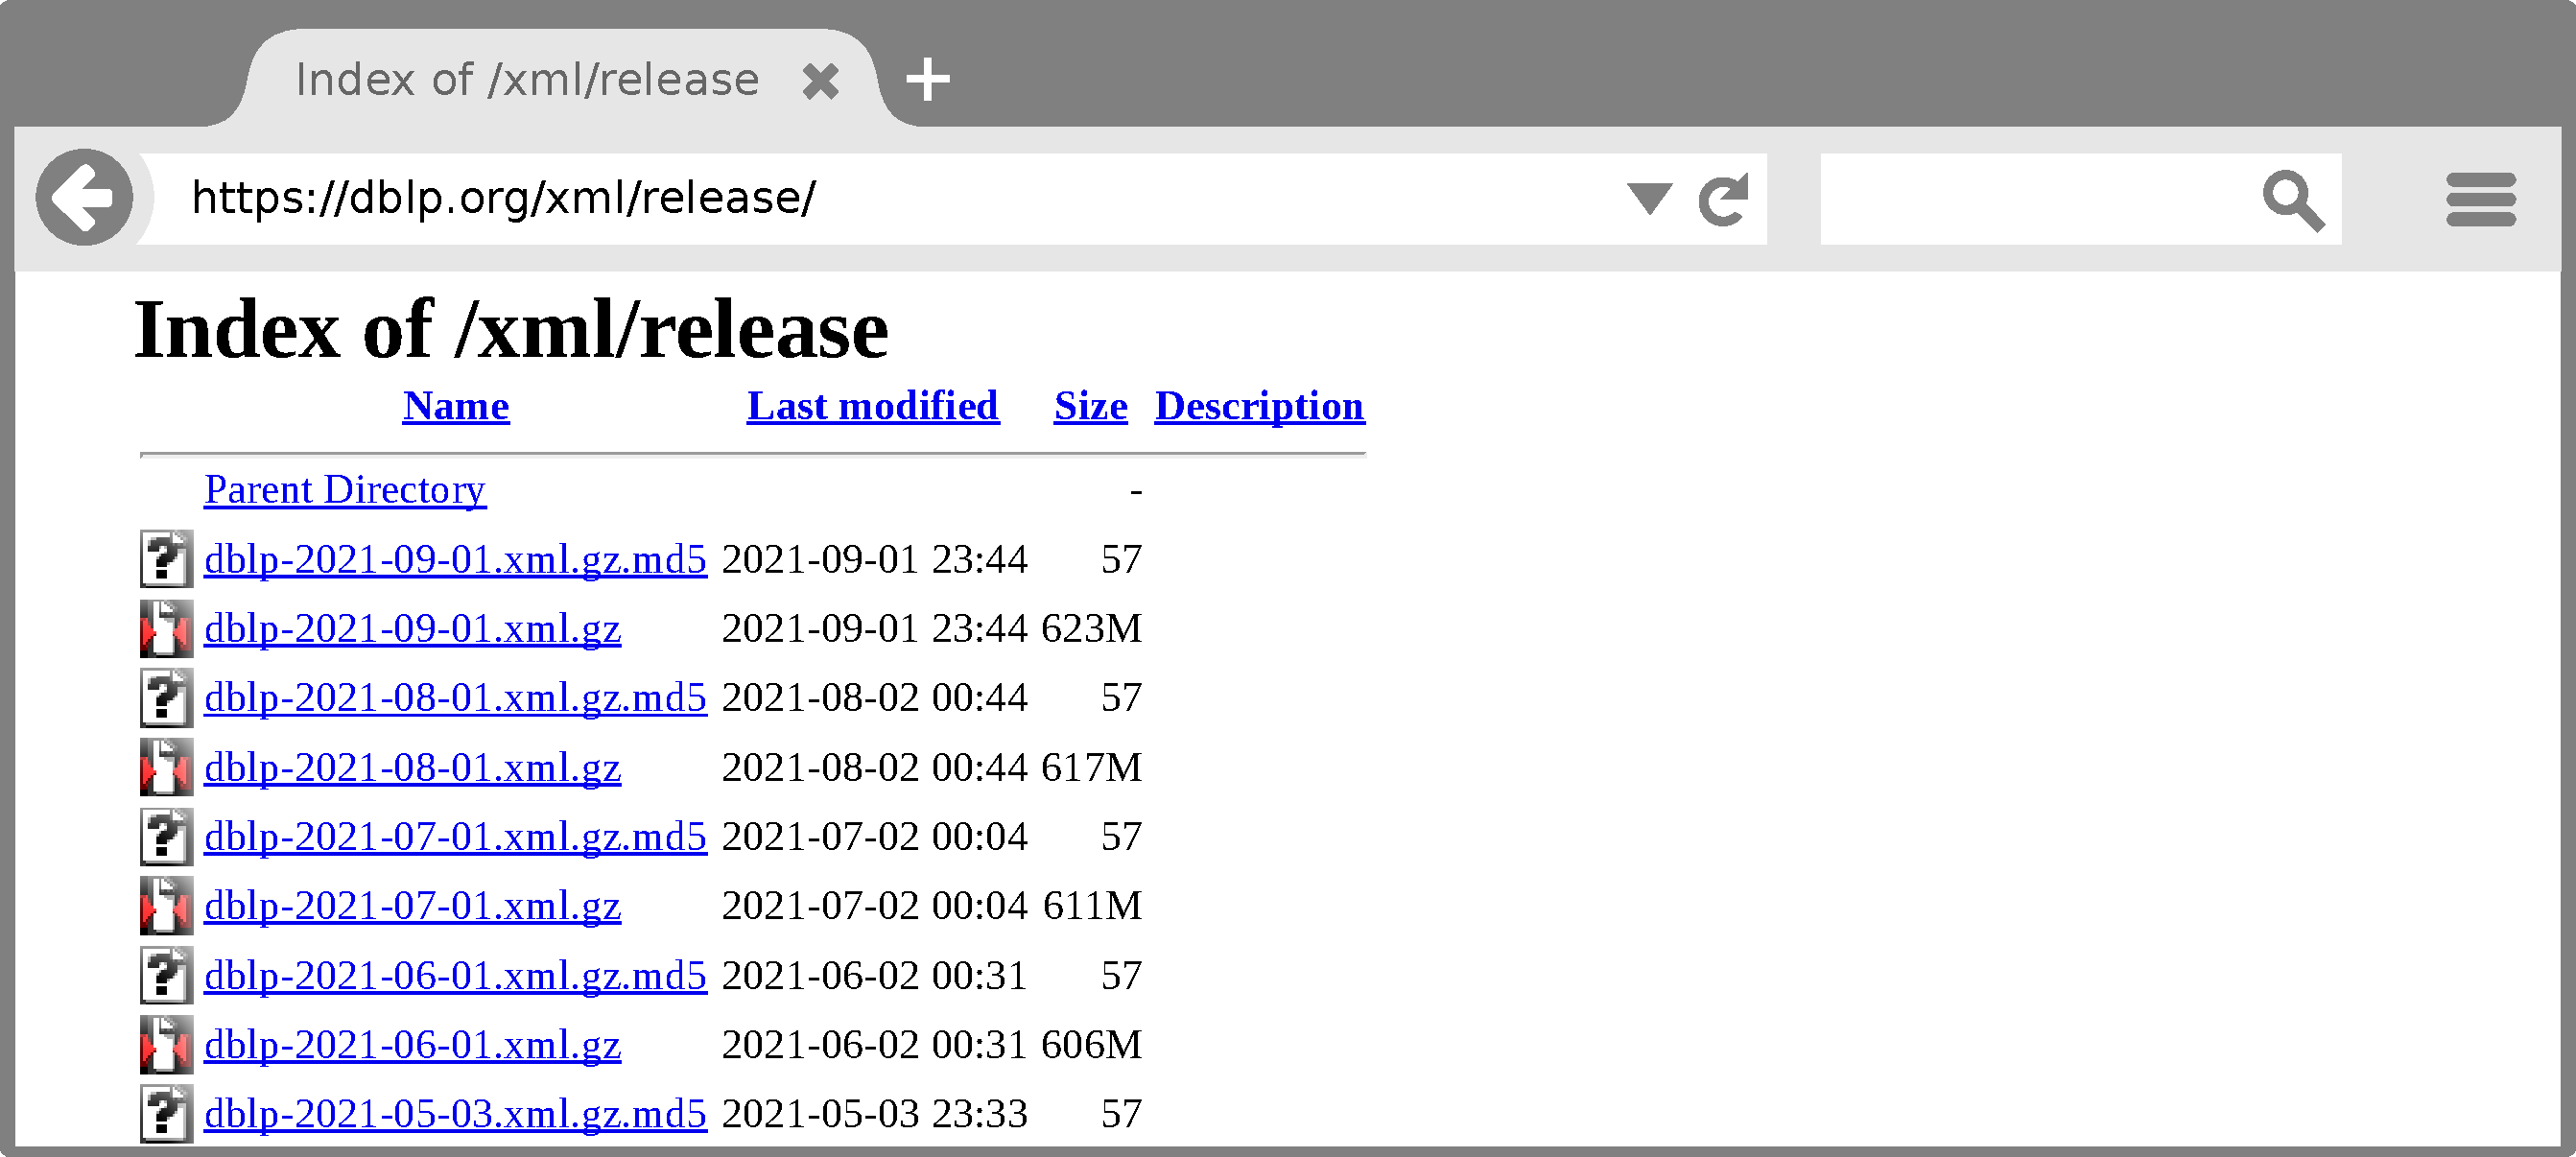
\includegraphics[width=1\textwidth]{images/chapter4/dblpdatasetdownload.pdf}%
	\caption[dblp dataset download]{\gls{dblp.org}\sfcite{Dagstuhl2021} dataset download}%
	\label{fig:dblpdatasetdownload}
\end{figure}%

As ArangoDB requires the data to be imported as JSON, more specifically single line JSON for a single document in a collection, the data has to be converted.
In the following paragraph data conversion is explained.
\bigskip

\noindent\textbf{Data conversion}

Because the dataset format does not correspond to the one accepted by ArangoDB for data import, the data needs to be converted from XML to JSON line format.

\noindent\lstinputlisting[
	%linerange = {1-29}, % choose line numbers to include
	language = XML,
	mathescape = true,
	label = {code:dblpdatasettop15lines},
	caption = {[An extract of dblp dataset, top 15 lines]An extract of \gls{dblp.org}\sfcite{Dagstuhl2021} dataset, top 15 lines}
]{code/dblpdatasettop15lines.xml}

From a first analysis of the contents of the extracted XML is possible to notice that the file in many (significantly) is not well formatted.
Many XML entries start right at the end of the previous ones without any empty line, or even without spaces - which makes it a hassle for parsers to directly parse the XML entries.

Another issue is that the extracted XML file is a little too large for a one go conversion. A splitting into smaller chunks is required too.

To solve these little problems, is proceeded in the following manner:
\setlist{nolistsep} \begin{enumerate}[noitemsep]
	\item A \gls{Python} script is written to clearly separate each XML entry from the previous and the next one with empty newlines.
	\item Another script is written to split the big XML file into smaller chunks of valid (not cut in half) XML entries.
	      The script splits to a new file every 1000000 lines (arbitrarily chosen).
	      If the millionth line cuts an XML entry in half, it will include the rest of the lines needed to complete that last XML entry for that chunk.
	\item A last script is written to convert each small chunk from XML to JSON.
	      \texttt{xmltodict} library is used to do the parsing and dumping of the converted JSON string.
\end{enumerate}

In \hyperref[longtable:dataconversion]{\autoref{longtable:dataconversion}} are shown the various scripts written to perform the needed data transformations.
For more, in the appendices see \hyperref[section:SourceCode/Projectrepositories]{\S\ \ref*{section:SourceCode/Projectrepositories}} 
%on \hyperref[section:SourceCode/Projectrepositories]{page \pageref*{section:SourceCode/Projectrepositories}}
and \hyperref[subsection:SourceCode/Instructionshowtorunbuildanddeploy/XMLtoJSONconversionscripts]{\S\ \ref*{subsection:SourceCode/Instructionshowtorunbuildanddeploy/XMLtoJSONconversionscripts}} on \hyperref[subsection:SourceCode/Instructionshowtorunbuildanddeploy/XMLtoJSONconversionscripts]{page \pageref*{subsection:SourceCode/Instructionshowtorunbuildanddeploy/XMLtoJSONconversionscripts}}.

\begin{center}
	\vspace*{-0.25cm}
	\begin{longtable}{p{0.47\linewidth}p{0.47\linewidth}}
		\hline \hline
		\textbf{Activity} & \textbf{Script's filename}\\
		\hline \hline
		\endfirsthead
		
		\multicolumn{2}{l}{... continued from previous page}\\
		\hline \hline
		\textbf{Activity} & \textbf{Script's filename}\\
		\hline \hline
		\endhead
		
		\hline
		\caption*{\tablename\ \thetable{}: \nameref*{longtable:dataconversion}. Continues on next page ...}
		\vspace*{0.5cm}
		\endfoot
		
		\hline
		%\multicolumn{2}{| c |}{End of Table}\\
		%\hline
		\caption{Scripts written for format correction, data splitting and conversion from XML to line JSON}\label{longtable:dataconversion}
		\vspace*{0.5cm}
		\endlastfoot

		XML format correction & \href{https://github.com/A-Domain-that-Rocks/convert_large_xml_to_json/blob/main/1_xml_to_xml_newlines.py}{\texttt{1\_xml\_to\_xml\_newlines.py}}%
		\footnote{\href{https://github.com/A-Domain-that-Rocks/convert_large_xml_to_json/blob/main/1_xml_to_xml_newlines.py}{\texttt{github.com/A-Domain-that-Rocks/convert\_large\_xml\_to\_json/blob/main/1\_xml\_to\_xml\_newlines.py}}}\\
		\hline
		XML splitting into smaller chunks & \href{https://github.com/A-Domain-that-Rocks/convert_large_xml_to_json/blob/main/2_split_xml_to_many_smaller_xml_files.py}{\texttt{2\_split\_xml\_to\_many\_smaller\_xml\_files.py}}%
		\footnote{\href{https://github.com/A-Domain-that-Rocks/convert_large_xml_to_json/blob/main/2_split_xml_to_many_smaller_xml_files.py}{\texttt{github.com/A-Domain-that-Rocks/convert\_large\_xml\_to\_json/blob/main/2\_split\_xml\_to\_many\_smaller\_xml\_files}}}\\
		\hline
		XML chunks conversion to line JSON entry chunks & \href{https://github.com/A-Domain-that-Rocks/convert_large_xml_to_json/blob/main/3_convert_xml_blocks_to_json_blocks.py}{\texttt{3\_convert\_xml\_blocks\_to\_json\_blocks.py}}%
		\footnote{\href{https://github.com/A-Domain-that-Rocks/convert_large_xml_to_json/blob/main/3_convert_xml_blocks_to_json_blocks.py}{\texttt{github.com/A-Domain-that-Rocks/convert\_large\_xml\_to\_json/blob/main/3\_convert\_xml\_blocks\_to\_json\_blocks.py}}}\\
		\hline
	\end{longtable}
	\vspace*{-1.35cm}
\end{center}

After having done the intermediate transformations and completed the conversion, is proceeded to the next phase: the importation of the line JSON data in an ArangoDB database' collection.

\subsection{Importing the data} \label{subsection:ImplementingtheWebApp/Thedata/Importingthedata}
\begin{figure}[H]%
	\centering%
	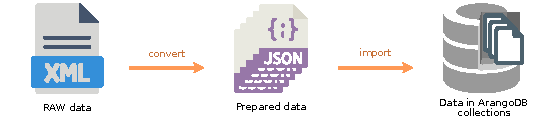
\includegraphics[width=1\textwidth,%
	]{images/chapter4/datatransformationsconvertimport.pdf}%
	\caption[Import of data in the database after conversion]{Import of data in the database after conversion}%
	\label{fig:datatransformationsconvertimport}%
\end{figure}%

In order to import the data in ArangoDB, firstly all the files containing JSON entries are copied to the DB host machine.

In \hyperref[longtable:dataimport]{\autoref{longtable:dataimport}} are shown the various scripts written to perform the movement of data files and then the import. For more, in the appendices see \hyperref[section:SourceCode/Projectrepositories]{\S\ \ref*{section:SourceCode/Projectrepositories}} on \hyperref[section:SourceCode/Projectrepositories]{page \pageref*{section:SourceCode/Projectrepositories}}
and \hyperref[subsection:SourceCode/Instructionshowtorunbuildanddeploy/CommandstoimporttheJSONdatainArangoDB]{\S\ \ref*{subsection:SourceCode/Instructionshowtorunbuildanddeploy/CommandstoimporttheJSONdatainArangoDB}} on \hyperref[subsection:SourceCode/Instructionshowtorunbuildanddeploy/CommandstoimporttheJSONdatainArangoDB]{page \pageref*{subsection:SourceCode/Instructionshowtorunbuildanddeploy/CommandstoimporttheJSONdatainArangoDB}}.

\begin{center}
	\vspace*{-0.25cm}
	\begin{longtable}{p{0.47\linewidth}p{0.47\linewidth}}
		\hline \hline
		\textbf{Activity} & \textbf{Script's filename}\\
		\hline \hline
		\endfirsthead
		
		\multicolumn{2}{l}{... continued from previous page}\\
		\hline \hline
		\textbf{Activity} & \textbf{Script's filename}\\
		\hline \hline
		\endhead
		
		\hline
		\caption*{\tablename\ \thetable{}: \nameref*{longtable:dataimport}. Continues on next page ...}
		\vspace*{0.5cm}
		\endfoot
		
		\hline
		%\multicolumn{2}{| c |}{End of Table}\\
		%\hline
		\caption{Scripts written for line JSON data import in ArangoDB}\label{longtable:dataimport}
		\vspace*{0.5cm}
		\endlastfoot

		Copy JSON files to database host machine & \href{https://github.com/A-Domain-that-Rocks/arangodb_import_json_data/blob/main/1_copy_json_to_DB_host_machine.sh}{\texttt{1\_copy\_json\_to\_DB\_host\_machine.sh}}%
		\footnote{\href{https://github.com/A-Domain-that-Rocks/arangodb_import_json_data/blob/main/1_copy_json_to_DB_host_machine.sh}{\texttt{github.com/A-Domain-that-Rocks/arangodb\_import\_json\_data/blob/main/1\_copy\_json\_to\_DB\_host\_machine.sh}}}\\
		\hline
		Import in ArangoDB & \href{https://github.com/A-Domain-that-Rocks/arangodb_import_json_data/blob/main/2_import_json_DB_to_arangodb.sh}{\texttt{2\_import\_json\_DB\_to\_arangodb.sh}}%
		\footnote{\href{https://github.com/A-Domain-that-Rocks/arangodb_import_json_data/blob/main/2_import_json_DB_to_arangodb.sh}{\texttt{github.com/A-Domain-that-Rocks/arangodb\_import\_json\_data/blob/main/2\_import\_json\_DB\_to\_arangodb.sh}}}\\
		\hline
	\end{longtable}
	\vspace*{-1.35cm}
\end{center}

Firstly a new database is created in ArangoDB - if the data will not be imported in \texttt{\_system}, the default autocreated DB during ArangoDB installation.
The ArangoDB user declared in the command for the importing of the data (see \hyperref[code:arangodbimportjsondata/2importjsonDBtoarangodb]{\autoref{code:arangodbimportjsondata/2importjsonDBtoarangodb}}) must have permissions setup correctly to do the said operations.
After that a collection is also created.
All this is information is given as arguments to the \texttt{arangoimport} command in the terminal.

\noindent\begin{minipage}{\linewidth} % Wraps the lstlisting inside a minipage of width \linewidth with no indentation to prevent it from splitting between pages
	\lstinputlisting[% will split at page breaks
		%linerange = {1-29}, % choose line numbers to include
		language = Bash,
		mathescape = false,
		label = {code:arangodbimportjsondata/2importjsonDBtoarangodb},
		caption = {[Bash command to import the JSON data ArangoDB using arangosh]Bash command to import the JSON data ArangoDB using arangosh\sfcite{ArangoDBarangoimport2021}}
	]{code/arangodbimportjsondata/2importjsonDBtoarangodb.sh}
\end{minipage}

The command is executed and once finished importing, the data in the collection is in the state shown in \hyperref[code:arangodbimportjsondata/2importjsonDBtoarangodb]{\autoref{code:arangodbimportjsondata/2importjsonDBtoarangodb}}. About 8.45 million documents are imported in total.

\begin{figure}[H]%
	\centering%
	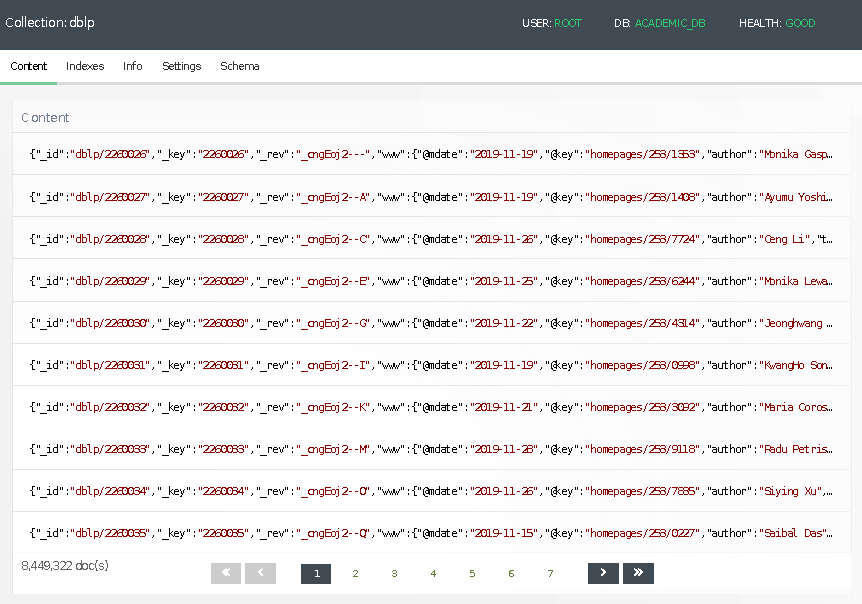
\includegraphics[%
		width=1\textwidth-4pt,%
		bgcolor=white,%
		cfbox=lightestgray % color
			  2pt % rule width
			  0pt % rule separation
			  0pt % margin
	]{images/chapter4/dblpcollectionafterimport.pdf}%
	\caption[Data in the dblp.org collection after the importation has finished]{Data in the \gls{dblp.org}\sfcite{Dagstuhl2021} collection after the importation has finished}%
	\label{fig:dblpcollectionafterimport}%
\end{figure}%

For a graph to be built with the data at hand, vertices and edges have to be defined. In the next subsection are presented the \glspl{data manipulation} performed to distribute the documents in collection into separate collections of vertices and edges.

\subsection{Transformations for vertex definitions} \label{subsection:ImplementingtheWebApp/Thedata/Transformationsforvertexdefinitions}
\begin{figure}[H]%
	\centering%
	
\includegraphics[width=1\textwidth,%
	]{images/chapter4/datatransformationsimporttransform.pdf}%
	\caption[Data transformations after import in order to obtain vertices]{Data transformations after import in order to obtain vertices}%
	\label{fig:datatransformationsimporttransform}%
\end{figure}%

Documents in the \gls{dblp.org}\sfcite{Dagstuhl2021} collection have to be separated and distributed in different collections, each representing the kind of vertex they semantically are. For example, publication documents will be collected in a collection called Publication, being vertices of that type. Authors shall be collected in a collection called Author, affiliation institutions in Institution and so on.

Most of the vertices aren't directly extractable from the data in the current form (see \hyperref[fig:arangodbwebinterfacedblpexampledocumenteditnew]{\autoref{fig:arangodbwebinterfacedblpexampledocumenteditnew}}). Some preprocessing has to be done in order to get separate collections for each kind of vertex, without duplicates and with the correct attributes in a well structured JSON document format.

\begin{figure}[H]%
	\centering%
	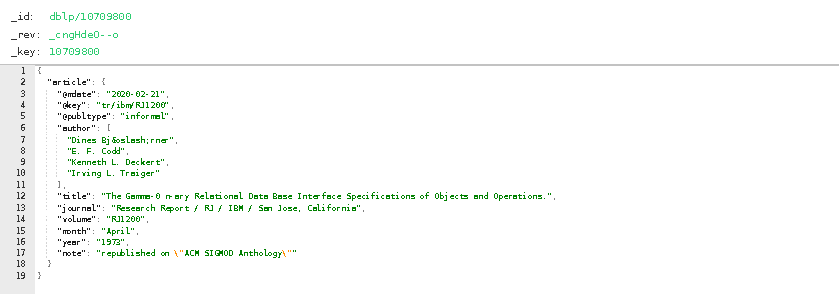
\includegraphics[%
		width=1\textwidth-4pt,%
		bgcolor=white,%
		cfbox=lightestgray % color
			  2pt % rule width
			  0pt % rule separation
			  0pt % margin
	]{images/chapter4/arangodbwebinterfacedblpexampledocumenteditnew.pdf}%
	\caption[Structure of documents from the imported data]{Structure of documents from the imported data}%
	\label{fig:arangodbwebinterfacedblpexampledocumenteditnew}%
\end{figure}%

The list of the files with the \acrshort{AQL} queries for the transformations and vertex document creations are reported in \hyperref[longtable:aqlqueriesvertices]{\autoref{longtable:aqlqueriesvertices}}).
For more, in the appendices see \hyperref[section:SourceCode/Projectrepositories]{\S\ \ref*{section:SourceCode/Projectrepositories}} on \hyperref[section:SourceCode/Projectrepositories]{page \pageref*{section:SourceCode/Projectrepositories}}
and \hyperref[subsection:SourceCode/Instructionshowtorunbuildanddeploy/AQLQueriestoeditcollectionscreatenodesedgesandgraphsfromtheimporteddata]{\S\ \ref*{subsection:SourceCode/Instructionshowtorunbuildanddeploy/AQLQueriestoeditcollectionscreatenodesedgesandgraphsfromtheimporteddata}} on \hyperref[subsection:SourceCode/Instructionshowtorunbuildanddeploy/AQLQueriestoeditcollectionscreatenodesedgesandgraphsfromtheimporteddata]{page \pageref*{subsection:SourceCode/Instructionshowtorunbuildanddeploy/AQLQueriestoeditcollectionscreatenodesedgesandgraphsfromtheimporteddata}}.
\medskip

During this process, in separated collections are created vertices of types: \texttt{author}, \texttt{publication}, \texttt{affiliated\_institution}, \texttt{journal}, \texttt{school}, \texttt{editor} and \texttt{publisher}.
Information on location was maintained as attributes of vertices that have it already.
It was not transformed into a separate type of vertex since very rarely present and even when there was information on location, it was in unstructured format.
Even in the case of affiliated institutions and schools, the case was somehow similar - even though less degenerated than locations with addresses and building numbers or only town names without any indication of countries...

\begin{center}
	\vspace*{-0.25cm}
	\begin{longtable}{p{0.47\linewidth}p{0.47\linewidth}}
		\hline \hline
		\textbf{Vertex type} & \textbf{\acrshort{AQL} query filename}\\
		\hline \hline
		\endfirsthead
		
		\multicolumn{2}{l}{... continued from previous page}\\
		\hline \hline
		\textbf{Vertex type} & \textbf{\acrshort{AQL} query filename}\\
		\hline \hline
		\endhead
		
		\hline
		\caption*{\tablename\ \thetable{}: \nameref*{longtable:aqlqueriesvertices}. Continues on next page ...}
		\vspace*{0.5cm}
		\endfoot
		
		\hline
		%\multicolumn{2}{| c |}{End of Table}\\
		%\hline
		\caption[AQL queries for the creation of vertex documents from the imported data]{\acrshort{AQL} queries for the creation of vertex documents from the imported data}\label{longtable:aqlqueriesvertices}
		\vspace*{0.5cm}
		\endlastfoot

		Author & \href{https://github.com/A-Domain-that-Rocks/distribute_data_in_arangodb/blob/main/02_create_author_nodes.aql}{\texttt{02\_create\_author\_nodes.aql}}\footnote{\href{https://github.com/A-Domain-that-Rocks/distribute\_data\_in\_arangodb/blob/main/02\_create\_author\_nodes.aql}{\texttt{github.com/A-Domain-that-Rocks/distribute\_data\_in\_arangodb/blob/main/02\_create\_author\_nodes.aql}}}\\
		\hline
		Publication & \href{https://github.com/A-Domain-that-Rocks/distribute_data_in_arangodb/blob/main/03_create_publication_nodes.aql}{\texttt{03\_create\_publication\_nodes.aql}}\footnote{\href{https://github.com/A-Domain-that-Rocks/distribute\_data\_in\_arangodb/blob/main/03\_create\_publication\_nodes.aql}{\texttt{github.com/A-Domain-that-Rocks/distribute\_data\_in\_arangodb/blob/main/03\_create\_publication\_nodes.aql}}}\\
		\hline
		Editor & \href{https://github.com/A-Domain-that-Rocks/distribute_data_in_arangodb/blob/main/08_create_editor_nodes.aql}{\texttt{08\_create\_editor\_nodes.aql}}\footnote{\href{https://github.com/A-Domain-that-Rocks/distribute\_data\_in\_arangodb/blob/main/08\_create\_editor\_nodes.aql}{\texttt{github.com/A-Domain-that-Rocks/distribute\_data\_in\_arangodb/blob/main/08\_create\_editor\_nodes.aql}}}\\
		\hline
		Publisher & \href{https://github.com/A-Domain-that-Rocks/distribute_data_in_arangodb/blob/main/10_create_publisher_nodes.aql}{\texttt{10\_create\_publisher\_nodes.aql}}\footnote{\href{https://github.com/A-Domain-that-Rocks/distribute\_data\_in\_arangodb/blob/main/10\_create\_publisher\_nodes.aql}{\texttt{github.com/A-Domain-that-Rocks/distribute\_data\_in\_arangodb/blob/main/10\_create\_publisher\_nodes.aql}}}\\
		\hline
		Series & \href{https://github.com/A-Domain-that-Rocks/distribute_data_in_arangodb/blob/main/12_create_series_nodes.aql}{\texttt{12\_create\_series\_nodes.aql}}\footnote{\href{https://github.com/A-Domain-that-Rocks/distribute\_data\_in\_arangodb/blob/main/12\_create\_series\_nodes.aql}{\texttt{github.com/A-Domain-that-Rocks/distribute\_data\_in\_arangodb/blob/main/12\_create\_series\_nodes.aql}}}\\
		\hline
		School & \href{https://github.com/A-Domain-that-Rocks/distribute_data_in_arangodb/blob/main/14_create_school_nodes.aql}{\texttt{14\_create\_school\_nodes.aql}}\footnote{\href{https://github.com/A-Domain-that-Rocks/distribute\_data\_in\_arangodb/blob/main/14\_create\_school\_nodes.aql}{\texttt{github.com/A-Domain-that-Rocks/distribute\_data\_in\_arangodb/blob/main/14\_create\_school\_nodes.aql}}}\\
		\hline
		Journal & \href{https://github.com/A-Domain-that-Rocks/distribute_data_in_arangodb/blob/main/24_create_journal_nodes.aql}{\texttt{24\_create\_journal\_nodes.aql}}\footnote{\href{https://github.com/A-Domain-that-Rocks/distribute\_data\_in\_arangodb/blob/main/24\_create\_journal\_nodes.aql}{\texttt{github.com/A-Domain-that-Rocks/distribute\_data\_in\_arangodb/blob/main/24\_create\_journal\_nodes.aql}}}\\
		\hline
	\end{longtable}
	\vspace*{-1.35cm}
\end{center}

\begin{remark}[on affiliated institutions and schools]\label{remark:onaffiliatedinstitutionsandschools}
    Should be noted that affiliated institutions and schools are created as different vertex types.
    This is done on purpose because in many publications with numerous authors, some authors have attributes of affiliations different from the institution where the main author teaches.
    Other reason is for example when a conference is organized in an institution and its proceedings affiliated to that institutions - but all the authors participating that conference are affiliated to other institutions different from the conference organizer's one.
    Because of this, these two vertices were maintained separate even though semantically school and institution are interchangeable.
\end{remark}

Once all the transformations have been performed, special ArangoDB edge collections will be used to store the edge documents linking millions of vertices.
This is the argument of the next subsection.

\subsection{Connecting the vertices with edges} \label{subsection:ImplementingtheWebApp/Thedata/Connectingtheverticeswithedges}
\begin{figure}[H]%
	\centering%
	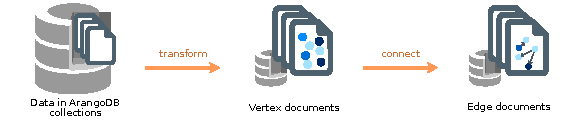
\includegraphics[width=1\textwidth,%
	]{images/chapter4/datatransformationstransformconnect.pdf}%
	\caption[Linking vertices with edges]{Linking vertices with edges}%
	\label{fig:datatransformationstransformconnect}%
\end{figure}%

In order to produce a graph, sets of vertices and edges linking them are needed.
Till now, with the various data transformations, only sets (of different types) of vertices have been produced.
To create connections between them, like "Author \texttt{HAS\_PUBLISHED} Publication" or "Publication \texttt{WAS\_CITED\_IN} Publication" and similar - special ArangoDB edge collection are used.
These collection force the use of documents with attributes specific to edges.
An edge document part of an edge collection has \texttt{\_to} and \texttt{\_from} attributes, used for creating a connection between the \texttt{\_id} of a vertex with one of another vertex.

The edge documents linking vertices are easily produced using \acrshort{AQL} queries.
The data involved are both the new vertex collections's produced in the previous subsection and the \gls{dblp.org}\sfcite{Dagstuhl2021} collection documents's.
\medskip

The list of the files with the queries for the edge creations are reported in \hyperref[longtable:aqlqueriesedges]{\autoref{longtable:aqlqueriesedges}}).


\begin{center}
	\vspace*{-0.25cm}
	\begin{longtable}{p{0.18875\linewidth}p{0.20275\linewidth}p{0.52350\linewidth}}
		\hline \hline
		\textbf{Vertex linked} & \textbf{to other vertex} & \textbf{\acrshort{AQL} query filename}\\
		\hline \hline
		\endfirsthead
		
		\multicolumn{2}{l}{... continued from previous page}\\
		\hline \hline
		\textbf{Vertex linked} & \textbf{to other vertex} & \textbf{\acrshort{AQL} query filename}\\
		\endhead
		
		\hline
		\caption*{\tablename\ \thetable{}: \nameref*{longtable:aqlqueriesedges}. Continues on next page ...}
		\vspace*{0.5cm}
		\endfoot
		
		\hline
		%\multicolumn{2}{| c |}{End of Table}\\
		%\hline
		\caption[AQL queries for the creation of edge documents linking pairs of vertex types]{\acrshort{AQL} queries for the creation of edge documents linking pairs of vertex types}\label{longtable:aqlqueriesedges}
		\vspace*{0.5cm}
		\endlastfoot

		Author & Publication & \href{https://github.com/A-Domain-that-Rocks/distribute_data_in_arangodb/blob/main/16_create_edges_between_author_and_publication_nodes.aql}{\texttt{16\_create\_edges\_between\_author\_and\newline\_publication\_nodes.aql}}\footnote{\href{https://github.com/A-Domain-that-Rocks/distribute\_data\_in\_arangodb/blob/main/16\_create\_edges\_between\_author\_and\_publication\_nodes.aql}{\texttt{github.com/A-Domain-that-Rocks/distribute\_data\_in\_arangodb/blob/main/\newline16\_create\_edges\_between\_author\_and\_publication\_nodes.aql}}}\\
		\hline
		Editor & Publication & \href{https://github.com/A-Domain-that-Rocks/distribute_data_in_arangodb/blob/main/17_create_edges_between_editor_and_publication_nodes.aql}{\texttt{17\_create\_edges\_between\_editor\_and\newline\_publication\_nodes.aql}}\footnote{\href{https://github.com/A-Domain-that-Rocks/distribute\_data\_in\_arangodb/blob/main/17\_create\_edges\_between\_editor\_and\_publication\_nodes.aql}{\texttt{github.com/A-Domain-that-Rocks/distribute\_data\_in\_arangodb/blob/main/\newline17\_create\_edges\_between\_editor\_and\_publication\_nodes.aql}}}\\
		\hline
		Publisher & Publication & \href{https://github.com/A-Domain-that-Rocks/distribute_data_in_arangodb/blob/main/20_create_edges_between_publisher_and_publication_nodes.aql}{\texttt{20\_create\_edges\_between\_publisher\_and\newline\_publication\_nodes.aql}}\footnote{\href{https://github.com/A-Domain-that-Rocks/distribute\_data\_in\_arangodb/blob/main/20\_create\_edges\_between\_publisher\_and\_publication\_nodes.aql}{\texttt{github.com/A-Domain-that-Rocks/distribute\_data\_in\_arangodb/blob/main/\newline20\_create\_edges\_between\_publisher\_and\_publication\_nodes.aql}}}\\
		\hline
		School & Publication & \href{https://github.com/A-Domain-that-Rocks/distribute_data_in_arangodb/blob/main/21_create_edges_between_school_and_publication_nodes.aql}{\texttt{21\_create\_edges\_between\_school\_and\newline\_publication\_nodes.aql}}\footnote{\href{https://github.com/A-Domain-that-Rocks/distribute\_data\_in\_arangodb/blob/main/21\_create\_edges\_between\_school\_and\_publication\_nodes.aql}{\texttt{github.com/A-Domain-that-Rocks/distribute\_data\_in\_arangodb/blob/main/\newline21\_create\_edges\_between\_school\_and\_publication\_nodes.aql}}}\\
		\hline
		Journal & Publication & \href{https://github.com/A-Domain-that-Rocks/distribute_data_in_arangodb/blob/main/36_create_edges_between_journal_and_publication_nodes.aql}{\texttt{36\_create\_edges\_between\_journal\_and\newline\_publication\_nodes.aql}}\footnote{\href{https://github.com/A-Domain-that-Rocks/distribute\_data\_in\_arangodb/blob/main/36\_create\_edges\_between\_journal\_and\_publication\_nodes.aql}{\texttt{github.com/A-Domain-that-Rocks/distribute\_data\_in\_arangodb/blob/main/\newline36\_create\_edges\_between\_journal\_and\_publication\_nodes.aql}}}\\
		\hline
		Series & Publication & \href{https://github.com/A-Domain-that-Rocks/distribute_data_in_arangodb/blob/main/37_create_edges_between_series_and_publication_nodes.aql}{\texttt{37\_create\_edges\_between\_series\_and\newline\_publication\_nodes.aql}}\footnote{\href{https://github.com/A-Domain-that-Rocks/distribute\_data\_in\_arangodb/blob/main/37\_create\_edges\_between\_series\_and\_publication\_nodes.aql}{\texttt{github.com/A-Domain-that-Rocks/distribute\_data\_in\_arangodb/blob/main/\newline37\_create\_edges\_between\_series\_and\_publication\_nodes.aql}}}\\
		\hline
		Affiliation institution & Author & \href{https://github.com/A-Domain-that-Rocks/distribute_data_in_arangodb/blob/main/38_create_edges_between_affiliation_institution_and_author_nodes.aql}{\texttt{38\_create\_edges\_between\_affiliation\_institution\_and\newline\_author\_nodes.aql}}\footnote{\href{https://github.com/A-Domain-that-Rocks/distribute\_data\_in\_arangodb/blob/main/38\_create\_edges\_between\_affiliation\_institution\_and\_author\_nodes.aql}{\texttt{github.com/A-Domain-that-Rocks/distribute\_data\_in\_arangodb/blob/main/\newline38\_create\_edges\_between\_affiliation\_institution\_and\_author\_nodes.aql}}}\\
		\hline
		Publication & Cited publication & \href{https://github.com/A-Domain-that-Rocks/distribute_data_in_arangodb/blob/main/39_create_edges_between_publication_and_cited_publication_nodes.aql}{\texttt{39\_create\_edges\_between\_publication\_and\newline\_cited\_publication\_nodes.aql}}\footnote{\href{https://github.com/A-Domain-that-Rocks/distribute\_data\_in\_arangodb/blob/main/39\_create\_edges\_between\_publication\_and\_cited\_publication\_nodes.aql}{\texttt{github.com/A-Domain-that-Rocks/distribute\_data\_in\_arangodb/blob/main/\newline39\_create\_edges\_between\_publication\_and\_cited\_publication\_nodes.aql}}}\\
		\hline
		Publication & Crossreffed publication & \href{https://github.com/A-Domain-that-Rocks/distribute_data_in_arangodb/blob/main/40_create_edges_between_publication_and_crossref-fed_publication_nodes.aql}{\texttt{40\_create\_edges\_between\_publication\_and\newline\_crossref-fed\_publication\_nodes.aql}}\footnote{\href{https://github.com/A-Domain-that-Rocks/distribute\_data\_in\_arangodb/blob/main/40\_create\_edges\_between\_publication\_and\_crossref-fed\_publication\_nodes.aql}{\texttt{github.com/A-Domain-that-Rocks/distribute\_data\_in\_arangodb/blob/main/\newline40\_create\_edges\_between\_publication\_and\_crossref-fed\_publication\_nodes.aql}}}\\
		\hline
	\end{longtable}
	\vspace*{-1.35cm}
\end{center}

After having produced all the edges linking the vertices, the view of the vertex and edge collections in the ArangoDB's web interface is as shown in \hyperref[fig:arangodbwebinterfacecollections]{\autoref{fig:arangodbwebinterfacecollections}}.
On the upper part of the figure are listed the vertex collections, with the exception of \gls{dblp.org}\sfcite{Dagstuhl2021}, \texttt{pub\_type} and \texttt{year} that are not used as vertices.
Whereas on the lower part of the figure are listed the edge collections.
The collections \texttt{author-author\_isnot}, \texttt{pub\_type-publication}, \texttt{year-publication} and \texttt{year-year} are not used.
These edge collections were produced but their value for the detection of communities was deemed neglectable.
For example, \texttt{author-author\_isnot} links an author to another author whose names are similar.
In the \gls{dblp.org}\sfcite{Dagstuhl2021} dataset this information is provided with an attribute of \texttt{isnot} taking as value the name of another author.
\medskip

In the next subsection, making use of the vertices and edges produced till now, the graph construction is presented.

\newpage
\begin{figure}[H]%
		\centering%
		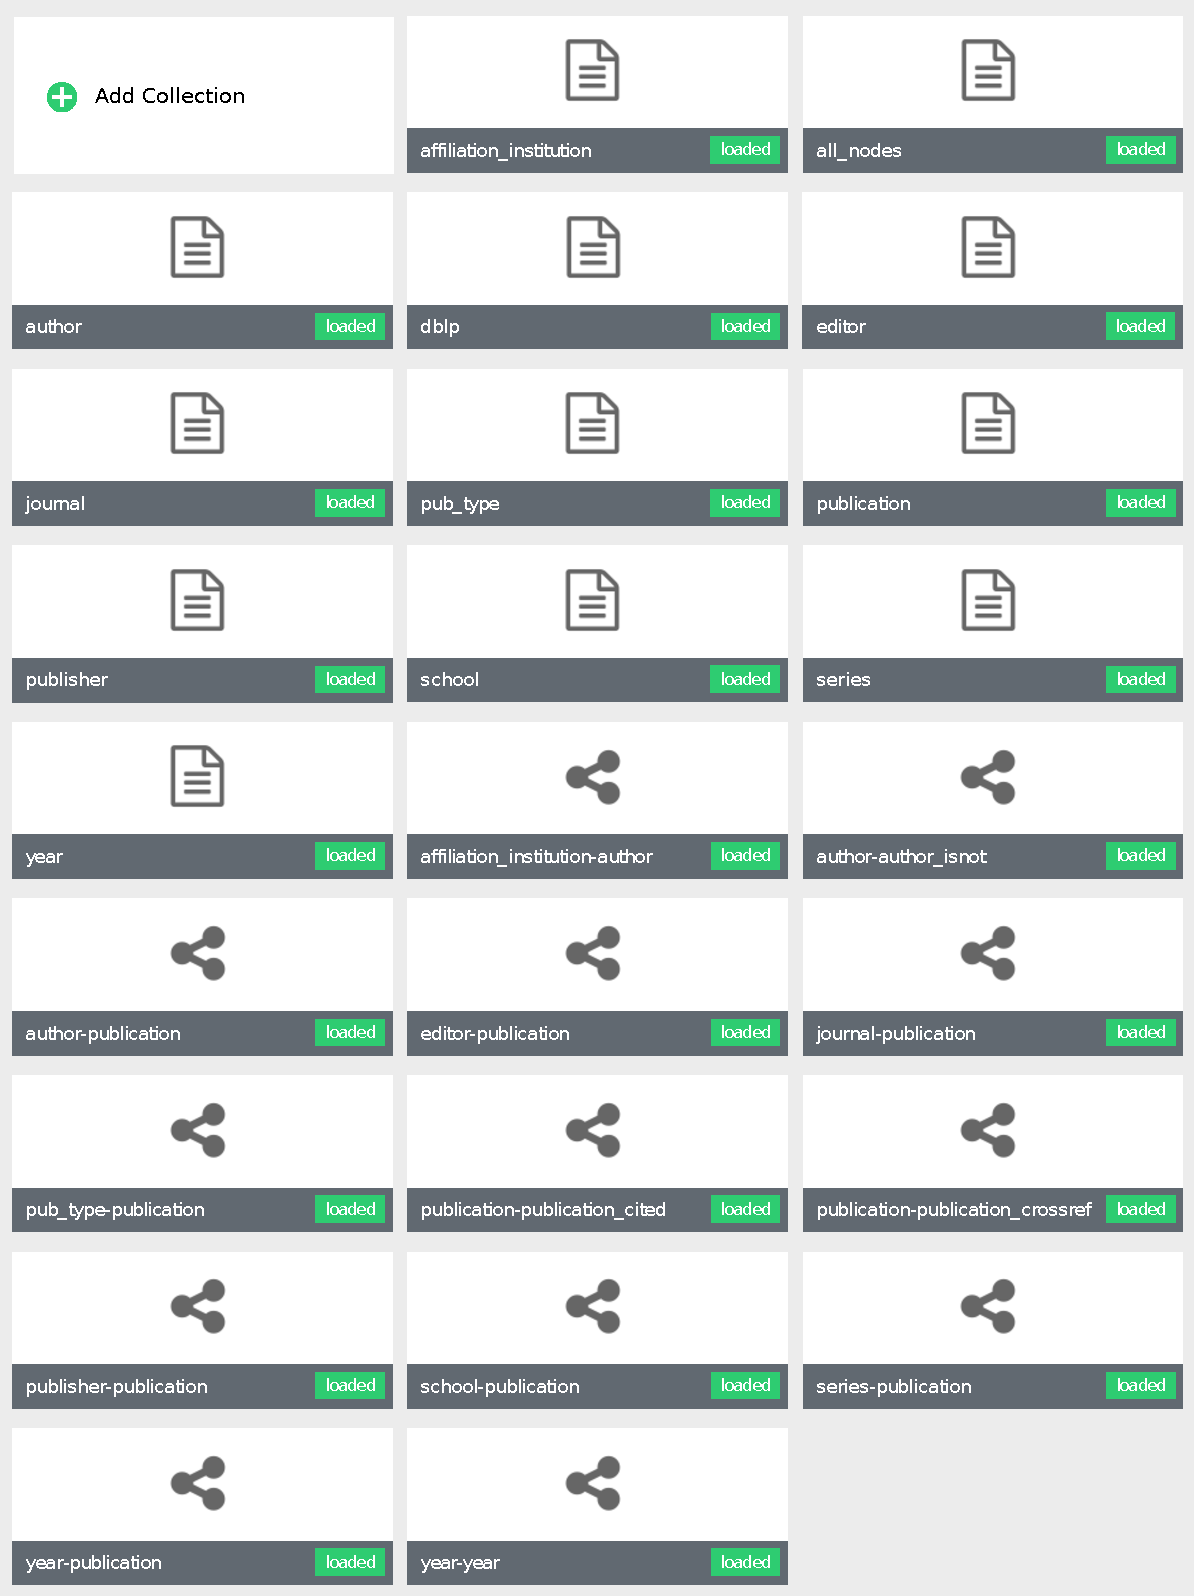
\includegraphics[%
			width=1\textwidth-4pt,%
			bgcolor=white,%
			cfbox=lightestgray % color
				  2pt % rule width
				  0pt % rule separation
				  0pt % margin
		]{images/chapter4/arangodbwebinterfacecollections.pdf}%
		\caption[Collections of vertices and edges in the ArangoDB web interface]{Collections of vertices and edges in the ArangoDB web interface}%
		\label{fig:arangodbwebinterfacecollections}%
\end{figure}%

\subsection{Building the scientific publications' graph} \label{subsection:ImplementingtheWebApp/Thedata/Buildingthescientificpublicationsgraph}
\begin{figure}[H]%
	\centering%
	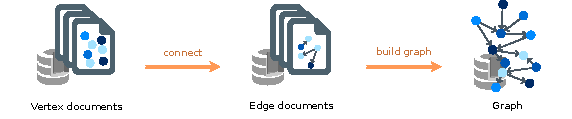
\includegraphics[width=1\textwidth,%
	]{images/chapter4/datatransformationsconnectbuildgraph.pdf}%
	\caption[Building the graph with the vertices and edges obtained in previous steps]{Building the graph with the vertices and edges obtained in previous steps}%
	\label{fig:datatransformationsconnectbuildgraph}%
\end{figure}%

Using the edge collections produced in the previous subsection, it is possible to build the graph of the scientific publications provided by \gls{dblp.org}\sfcite{Dagstuhl2021}.
ArangoDB obtains the set of vertices of the graph from the \_to and \_from fields of each edge document.

The final graph is shown in \hyperref[fig:SnapshotArangoDBGraphPrevidiMazzolenishort]{\S\ \ref*{fig:SnapshotArangoDBGraphPrevidiMazzolenishort}}.
Arrived at this point, it is possible to detect the communities as described in \hyperref[section:CommunityDetection/ClusteringcollaborationcommunitiesAlgorithmexecution]{\S\ \ref*{section:CommunityDetection/ClusteringcollaborationcommunitiesAlgorithmexecution}} on \hyperref[section:CommunityDetection/ClusteringcollaborationcommunitiesAlgorithmexecution]{page \pageref*{section:CommunityDetection/ClusteringcollaborationcommunitiesAlgorithmexecution}} or go on with the development of the \gls{Web Application}'s backend \acrshort{API} (see \hyperref[section:ImplementingtheWebApp/TheAPI]{\S\ \ref*{section:ImplementingtheWebApp/TheAPI}} on \hyperref[section:ImplementingtheWebApp/TheAPI]{page \pageref*{section:ImplementingtheWebApp/TheAPI}}) and frontend UI (see \hyperref[section:ImplementingtheWebApp/Thefrontend]{\S\ \ref*{section:ImplementingtheWebApp/Thefrontend}} on \hyperref[section:ImplementingtheWebApp/Thefrontend]{page \pageref*{section:ImplementingtheWebApp/Thefrontend}}).

\begin{figure}[H]%
		\centering%
		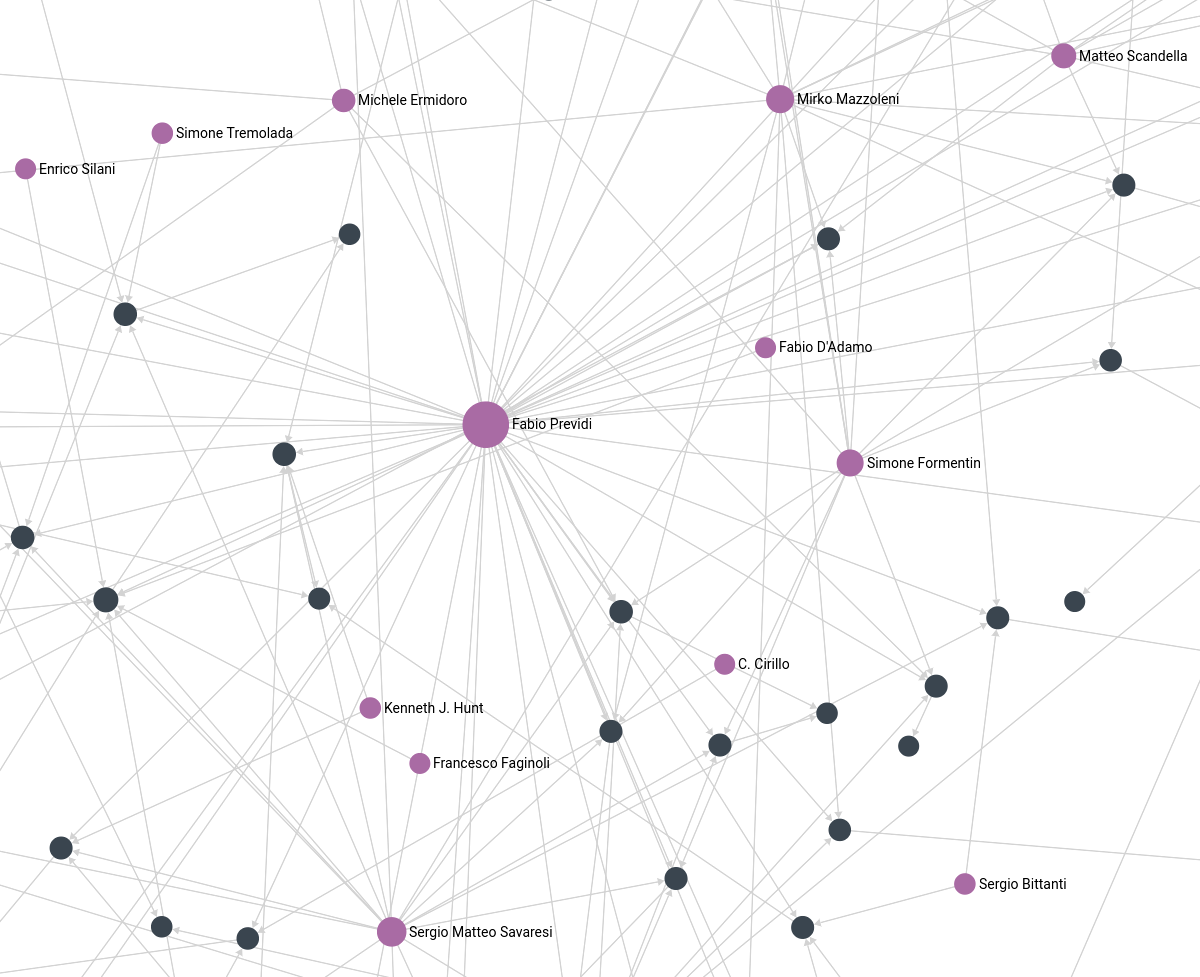
\includegraphics[%
			width=1\textwidth-4pt,%
			bgcolor=white,%
			cfbox=lightestgray % color
				  2pt % rule width
				  0pt % rule separation
				  0pt % margin
		]{images/chapter4/SnapshotArangoDBGraphPrevidiMazzolenishort.png}%
		\caption[The graph built after all the data manipulations - Vertices shown: Prof. Previdi, Mazzoleni, Ermidoro, Scandella and even Prof. Bittanti]{The graph built after all the \gls{data manipulation}s - Vertices shown: Prof. Previdi, Mazzoleni, Ermidoro, Scandella and Prof. Bittanti}%
		\label{fig:SnapshotArangoDBGraphPrevidiMazzolenishort}%
\end{figure}%

\section[The API]{The \acrshort{API}} \label{section:ImplementingtheWebApp/TheAPI}
\begin{figure}[H]%
		\centering%
		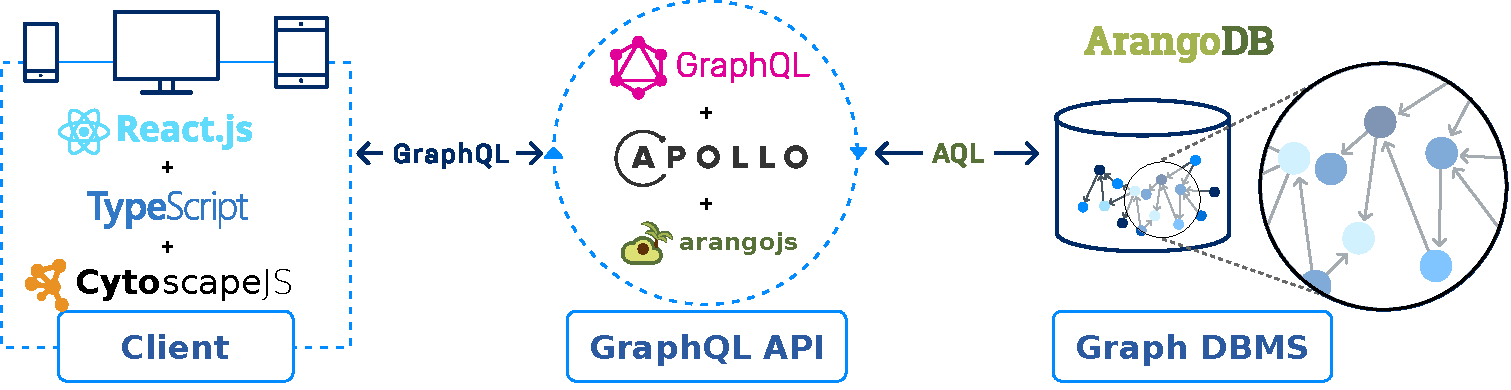
\includegraphics[width=1\textwidth]{images/chapter4/architecture.pdf}%
		\caption[Architecture of the Web Application]{Architecture of the \gls{Web Application}}%
		\label{fig:architecture}%
\end{figure}%

In this section is described the implementation of an initially Rest and then \gls{GraphQL} \gls{APIg} for querying the ArangoDB Graph Database from the website's frontend, or even other clients.

At its final state, the implemented server uses NodeJS, \gls{Express}, \gls{GraphQL} and \gls{Apollo Server} to serve its functionalities.

\subsection[Implementing a NodeJS \& Express simple Rest API server]{Implementing a NodeJS \& \gls{Express} simple Rest \acrshort{API} server} \label{subsection:ImplementingtheWebApp/TheAPI/Implementing a NodeJSExpresssimpleRestAPIserver}
Initially, the backend of the \gls{Web Application} is developed as a traditional Rest \acrshort{API}.
It is done this way because of the greater familiarity with this type of \acrshort{API} and for getting then started straightahead with the development of the frontend interface.

NodeJS and \gls{Express} are used.
See \hyperref[section:SourceCode/Projectrepositories]{\S\ \ref{section:SourceCode/Projectrepositories}} for source code and \hyperref[subsection:SourceCode/Instructionshowtorunbuildanddeploy/Backendssourcecode]{\S\ \ref{subsection:SourceCode/Instructionshowtorunbuildanddeploy/Backendssourcecode}} for instructions on how to get the source code, run and deploy it.

The built \acrshort{API}, at user request from the frontend or from any \acrshort{API} querying client, responds with vertex IDs in the case of the search form with autocomplete suggestions - and with vertex and edge data when a specific graph is requested.

\noindent\begin{minipage}{\linewidth} % Wraps the lstlisting inside a minipage of width \linewidth with no indentation to prevent it from splitting between pages
	\noindent\lstinputlisting[% will split at page breaks
		%linerange = {1-29}, % choose line numbers to include
		language = JavaScript,
		mathescape = false,
		label = {code:adomainthatrocksbackend/servicerest},
		caption = {[Rest API's service]Rest API's service}
	]{code/adomainthatrocksbackend/servicerest.js}
\end{minipage}

At this stage, no information on detected communities is sent in responses.
Once the frontend shall be at a development stage to display compound nodes, detected communities' data will be included in the responses.

Once developed a minimal Web App consisting of DB + backend with Rest \acrshort{API} + basic frontend, the \acrshort{API} is upgraded to a GraphQL + \gls{Apollo Server} \acrshort{API}. This is presented in the next subsection.

\subsection[Moving towards a GraphQL API]{Moving towards a \gls{GraphQL} \acrshort{API}} \label{subsection:ImplementingtheWebApp/TheAPI/MovingtowardsaGraphQLAPI}
\begin{figure}[H]%
		\centering%
		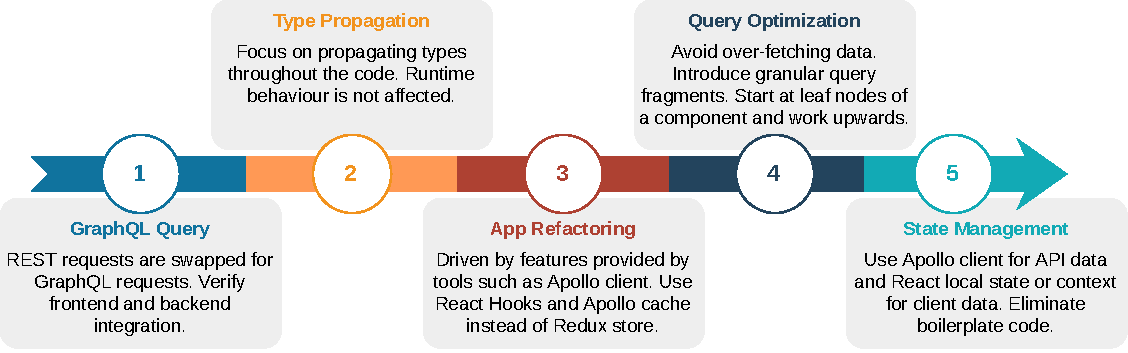
\includegraphics[width=1\textwidth]{images/chapter4/graphqlapollo.pdf}%
		\caption[A typical transition from Rest to an API with GraphQL and Apollo]{A typical transition from Rest to an \acrshort{API} with \gls{GraphQL} and \gls{Apollo}}%
		\label{fig:graphqlapollo}%
\end{figure}%

\gls{GraphQL} is an open-source data query and manipulation language for \acrshort{API}s.
It also serves as a runtime for fulfilling queries.
\gls{GraphQL} was developed at \gls{Facebook} and was publicly released in 2015.
It is chosen to develop the \acrshort{API} with it because of a variety of (good) reasons - having the word "graph" in its name is not one of them.

\begin{quoting}[
	begintext={},
	endtext={ - \gls{GraphQL}}
]
	\centering\textit{"Ask for what you need, get exactly that"}
\end{quoting}

While Rest \acrshort{API}s require querying multiple URLs/routes for different data, \gls{GraphQL} \acrshort{API}s get all the data in a single request.
Differently from the many endpoints of a typical Rest \acrshort{API}, \gls{GraphQL} \acrshort{API}s make use of a type system consisting of types and fields to ensure an app only asks for what's offered and provide clear and helpful errors.
Also using types avoids the need to write manual parsing functionalities.

Along with \gls{GraphQL}, \gls{Apollo} is used.
\gls{Apollo Server} is an open-source, spec-compliant \gls{GraphQL} server that is compatible with any \gls{GraphQL client}.
It's the best way to build a production-ready, self-documenting \gls{GraphQL} \acrshort{API} that can use data from any source.

\noindent\begin{minipage}{1\linewidth} % Wraps the lstlisting inside a minipage of width \linewidth with no indentation to prevent it from splitting between pages
    \noindent\lstinputlisting[% will split at page breaks
    	%linerange = {1-29}, % choose line numbers to include
    	language = JavaScript,
    	mathescape = false,
    	label = {code:adomainthatrocksbackend/servergraphql},
    	caption = {[Part of the code of the API server with GraphQL and Apollo]Part of the code of the \acrshort{API} server with \gls{GraphQL} and \gls{Apollo}}
    ]{code/adomainthatrocksbackend/servergraphql.js}
\end{minipage}

A \gls{GraphQL} and \gls{Apollo} \acrshort{API} was implemented (with some basic resolver functions) and their integration with ArangoDB, a graph DBMS (at least for this thesis purposes) - was tested.
Everything communicates flawlessly and the responses are as intended.

At migration concluded from the Rest \acrshort{API} to the \gls{GraphQL} \acrshort{API} with \gls{Apollo}, the code is as shown in \hyperref[code:adomainthatrocksbackend/servergraphql]{\autoref{code:adomainthatrocksbackend/servergraphql}}.
For the \gls{GraphQL schema} with the type (and their fields) definitions, see \hyperref[code:adomainthatrocksbackend/graphql/schema]{\autoref{code:adomainthatrocksbackend/graphql/schema}} in \hyperref[appendix:APIDocs]{appendix \S\ B} on \hyperref[code:adomainthatrocksbackend/graphql/schema]{page \pageref*{code:adomainthatrocksbackend/graphql/schema}}.
For the resolvers, implemented functions' source code and how to get them running, see \hyperref[appendix:SourceCode]{appendix \S\ A} on \hyperref[subsection:SourceCode/Instructionshowtorunbuildanddeploy/Backendssourcecode]{page \pageref*{subsection:SourceCode/Instructionshowtorunbuildanddeploy/Backendssourcecode}}.

\subsection{Resolvers}\label{subsection:ImplementingtheWebApp/TheAPI/Resolvers}
The \acrshort{API} needs to handle two types of requests:
\setlist{nolistsep} \begin{enumerate}[noitemsep]
	\item request for the ids (and names) of nodes named similarly to a given string;
	\item graph data request (nodes, edges communities) given a vertex id and min, max number of hops.
\end{enumerate}

Follows why and how these requests are handled.

\noindent\begin{minipage}{1\linewidth} % Wraps the lstlisting inside a minipage of width \linewidth with no indentation to prevent it from splitting between pages
	\lstinputlisting[% will split at page breaks
		%linerange = {1-29}, % choose line numbers to include
		language = JavaScript,
		mathescape = false,
		label = {code:adomainthatrocksbackend/resolvers},
		caption = {[GraphQL API's resolvers changed version after frontend implementation]\gls{GraphQL} \acrshort{API}'s resolvers changed version after frontend implementation}
	]{code/adomainthatrocksbackend/resolvers.js}
\end{minipage}

\subsubsection{Autocomplete suggestion query for string to ID translation}\label{subsubsection:ImplementingtheWebApp/TheAPI/Resolvers/AutocompletesuggestionqueryforstringtoIDtranslation}
In short, the user from the frontend inserts three inputs that indicate which entity's collaboration graph to display and how far (how many hops) from that entity to look for other entities (min and max depth).\label{tobementionedthefrontendthreeinputs}
In terms of information to include in the query, this translates to a string representing the name or title of the entity/vertex (author, publication, institution etc.), a number for the minimum depth and another number for the maximum depth.

Since naming is a difficult problem, the string representing the name or title of the start vertex has to refer to exactly one vertex of the graph - otherwise the graph traversal cannot be performed since the startnode's identifying string would not be deterministic.

To solve this, it is needed to make a translation from the user's input string - that is a name, be it an author's name or a publication title or some institutions name - into an id corresponding exactly to one document in the database collections, the startNode vertex document.\label{tobementionedthefrontendtranslationnametoid}
Making use of autocomplete suggestions in the search form, a user's input in the form field queries the \acrshort{API} for vertices named in a similar way to that string.
The \acrshort{API} then queries the database sending a specific \acrshort{AQL} query to obtain possible vertices that match the user's input.
In the response to the frontend, the \acrshort{API} sends the full names/titles of the vertices similar to the string the user wrote - and these vertices IDS.
The search form then displays these elements to the user as a list of suggestions (selectable vertices) so he/she can select one.
The selected vertex's ID is used, once the user has inserted the min and max depth too, to form an exact (deterministic) query that the \acrshort{API} sends to the DB.
That query is non-ambiguous since IDs are unique. It would not have been like that if names/title were used to refer to vertices.

\begin{figure}[H]%
		\centering%
		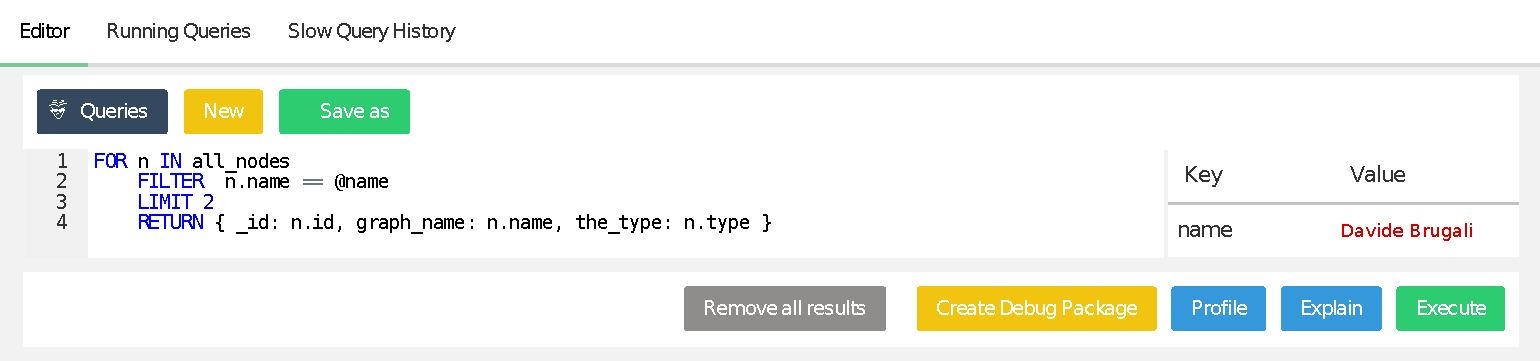
\includegraphics[%
			width=1\textwidth-4pt,%
			bgcolor=white,%
			cfbox=lightestgray % color
				  2pt % rule width
				  0pt % rule separation
				  0pt % margin
		]{images/chapter4/QueryResolverSearchFormAutocompleteBrugali.pdf}%
		\caption[Execution in ArangoDB of backend resolver's AQL query for search form autocomplete suggestions. String: "Davide Brugali"]{Execution in ArangoDB of \gls{backend} resolver's \acrshort{AQL} query for search form autocomplete suggestions. String: "Davide Brugali"}%
		\label{fig:QueryResolverSearchFormAutocompleteBrugali}%
\end{figure}%

In \hyperref[fig:QueryResolverSearchFormAutocompleteBrugali]{\autoref{fig:QueryResolverSearchFormAutocompleteBrugali}} is shown the \acrshort{API}'s \acrshort{AQL} query for autocomplete suggestions (translations from string name/title to unique ID of a vertex of the graph) executed directly in the ArangoDB database's web interface.
The found results shown in \hyperref[fig:QueryResolverSearchFormAutocompleteBrugaliResponseJSON]{\autoref{fig:QueryResolverSearchFormAutocompleteBrugaliResponseJSON}}, in the same fashion are sent to the \acrshort{API} - which then forwards them to the frontend interface.

\begin{figure}[H]%
		\centering%
		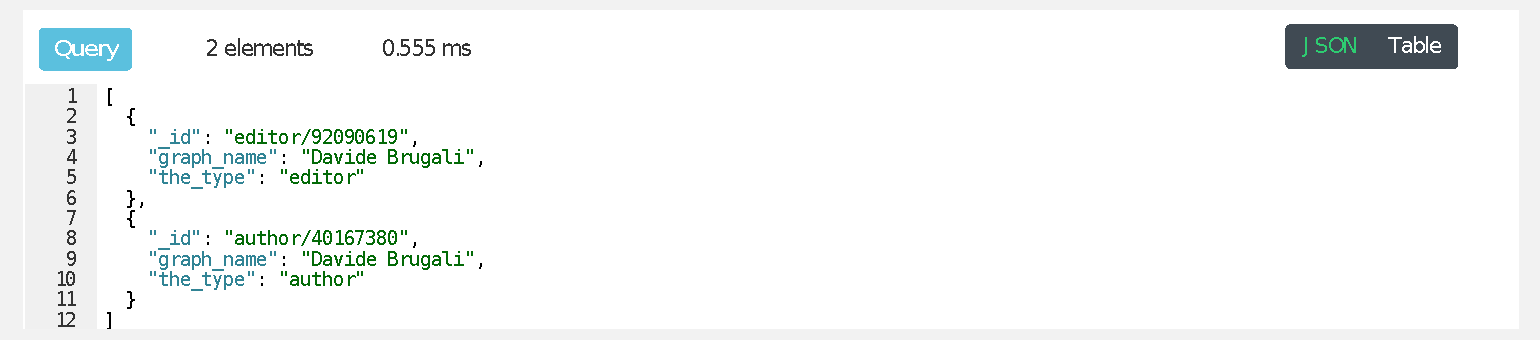
\includegraphics[%
			width=1\textwidth-4pt,%
			bgcolor=white,%
			cfbox=lightestgray % color
				  2pt % rule width
				  0pt % rule separation
				  0pt % margin
		]{images/chapter4/QueryResolverSearchFormAutocompleteBrugaliResponseJSON.pdf}%
		\caption[Result of the query execution displayed in \autoref*{fig:QueryResolverSearchFormAutocompleteBrugali}]{Result of the query execution displayed in \hyperref[fig:QueryResolverSearchFormAutocompleteBrugali]{\autoref{fig:QueryResolverSearchFormAutocompleteBrugali}}}%
		\label{fig:QueryResolverSearchFormAutocompleteBrugaliResponseJSON}%
\end{figure}%
\medskip

It is now clear why the needed queries (thus resolver functions) are two:
one for name to ID translation just presented and the second one for requesting collaboration graph nodes, vertices and communities data.
The second resolver is reported below.

\subsubsection{Querying for graph data}\label{subsubsection:ImplementingtheWebApp/TheAPI/Resolvers/Queryingforgraphdata}
With two resolvers and many types (see \hyperref[code:adomainthatrocksbackend/graphql/schema]{\autoref{code:adomainthatrocksbackend/graphql/schema}} in \hyperref[appendix:APIDocs]{appendix \S\ B} on \hyperref[code:adomainthatrocksbackend/graphql/schema]{page \pageref*{code:adomainthatrocksbackend/graphql/schema}}) defined as the different vertices (\texttt{author}, \texttt{publication}, \texttt{affiliation\_institution}, \texttt{publisher}, \texttt{editor}, ...) - the \acrshort{API} manages to get queries from the frontend, create \acrshort{AQL} queries to send to the DB and forward the response data back to the frontend.

The graph data requiring query is handled by a resolver function that builds an \acrshort{AQL} query using the translated ID and the depth inputs of the user and sends it to the database in order to perform a graph traversal.

In \hyperref[fig:QueryResolverGraphBrugali]{\autoref{fig:QueryResolverGraphBrugali}}, the ID of the author found in the previous query is used as input in this new query along with the min and max depth.
The query returns the graph data consisting of the nodes, edges and communities (compound nodes) the derived number of hops distant from the start node.
In the ArangoDB's web interface, when a query's result is made of nodes and edges, that result's data is sufficient for ArangoDB to automatically render a graph (see \hyperref[fig:QueryResolverGraphBrugaliResponseGraph]{\autoref{fig:QueryResolverGraphBrugaliResponseGraph}}).
The response returned is of course in JSON format consisting of:
\setlist{nolistsep} \begin{itemize}[noitemsep]
	\item a startNode vertex, corresponding to the vertex id given in input;
	\item a list of distinct vertices composing the graph;
	\item a list of the edges connecting the vertices of the graph;
	\item a list of the communities the nodes of the graph belong to.
\end{itemize}

These resolver functions are sufficient to provide the data needed to build graphs in the frontend.

\begin{figure}[H]%
		\centering%
		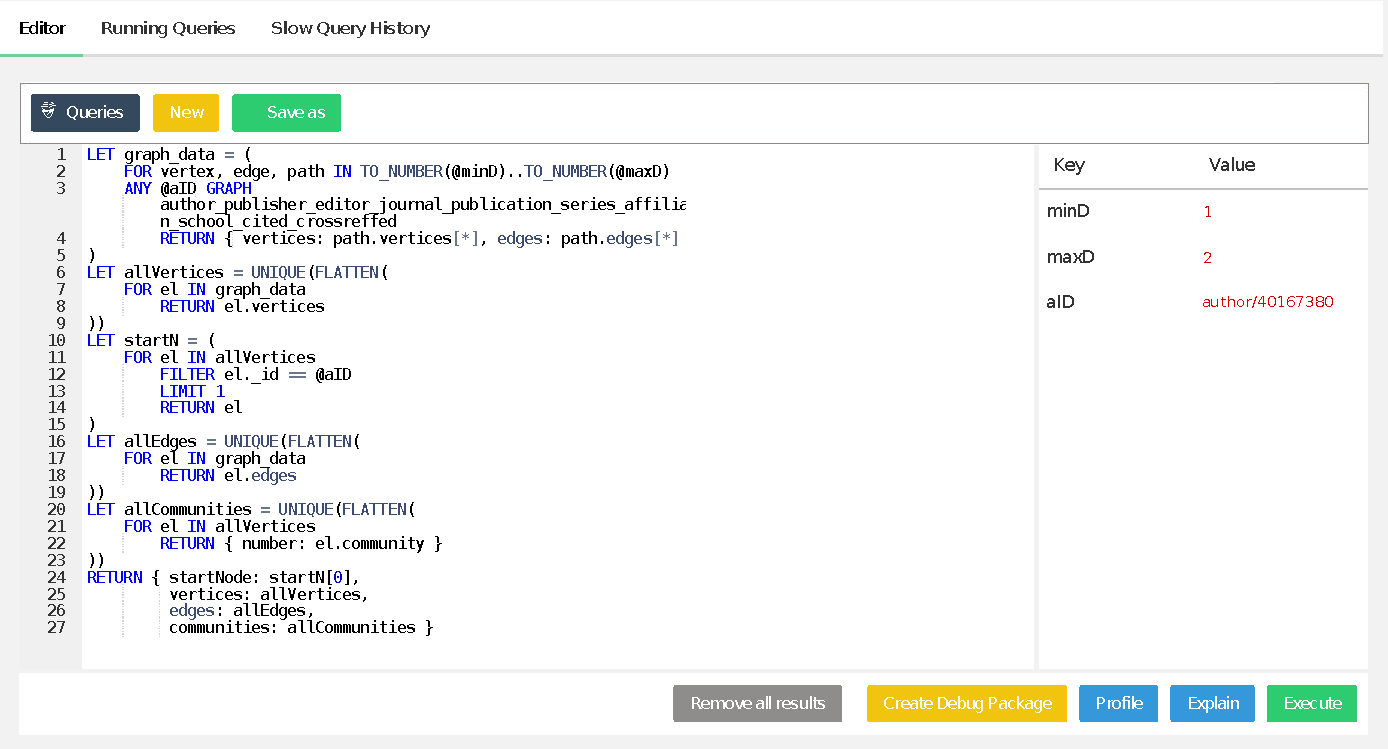
\includegraphics[%
			width=1\textwidth-4pt,%
			bgcolor=white,%
			cfbox=lightestgray % color
				  2pt % rule width
				  0pt % rule separation
				  0pt % margin
		]{images/chapter4/QueryResolverGraphBrugali.pdf}%
		\caption[Execution in ArangoDB of backend resolver's AQL query for graph data retrieval]{Execution in ArangoDB of \gls{backend} resolver's \acrshort{AQL} query for graph data retrieval}%
		\label{fig:QueryResolverGraphBrugali}%
\end{figure}%

\begin{figure}[H]%
		\centering%
		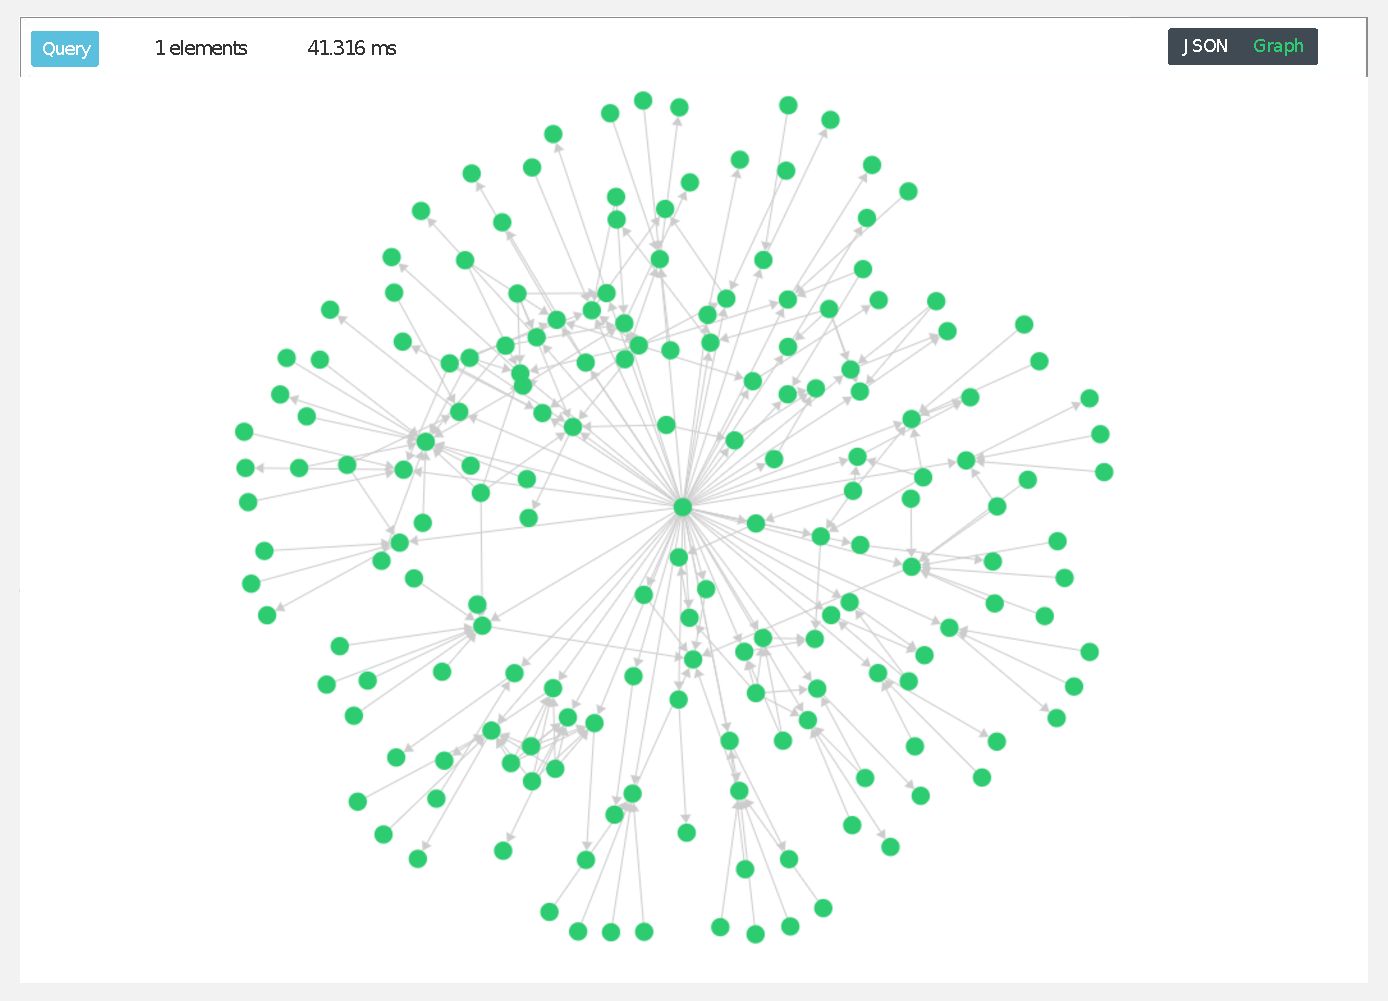
\includegraphics[%
			width=1\textwidth-4pt,%
			bgcolor=white,%
			cfbox=lightestgray % color
				  2pt % rule width
				  0pt % rule separation
				  0pt % margin
		]{images/chapter4/QueryResolverGraphBrugaliResponseGraph.pdf}%
		\caption[Result of the query execution displayed in \autoref*{fig:QueryResolverGraphBrugali}]{Result of the query execution displayed in \hyperref[fig:QueryResolverGraphBrugali]{\autoref{fig:QueryResolverGraphBrugali}}}%
		\label{fig:QueryResolverGraphBrugaliResponseGraph}%
\end{figure}%

In the next section is presented the development of the frontend interface and how the data from the \acrshort{API} are used.

\section{The frontend} \label{section:ImplementingtheWebApp/Thefrontend}
In this section are presented the implementation details of the frontend of the WebApp from its creation from a Typescript template to rendering graphs and communities within it.

\subsection{Creating a simple React \& TypeScript project} \label{subsection:ImplementingtheWebApp/Thefrontend/CreatingasimpleReactTypescriptproject}
As shown in \hyperref[fig:architecture]{\autoref{fig:architecture}} on \hyperref[fig:architecture]{page \pageref*{fig:architecture}}, the frontend is made using React, TypeScript and \gls{Apollo Client} - even though TypeScript is used not the way it is intended to be used.
\texttt{\gls{Cytoscape.JS}} library is used for graph rendering and \texttt{\Gls{bootstrap}} for styling.
See \hyperref[section:SourceCode/Projectrepositories]{\S\ \ref{section:SourceCode/Projectrepositories}} for source code and \hyperref[subsection:SourceCode/Instructionshowtorunbuildanddeploy/Frontendssourcecode]{\S\ \ref{subsection:SourceCode/Instructionshowtorunbuildanddeploy/Frontendssourcecode}} for instructions on how to get the source code, run, build and deploy it.

The features/functionalities/components the frontend interface needs are two:
\setlist{nolistsep} \begin{itemize}[noitemsep]
	\item a search form component to give the user the possibility to search for some entities collaboration network,
	\item and a graph rendering component in order to display the graph that was searched for.
\end{itemize}

\begin{figure}[H]%
	\centering%
	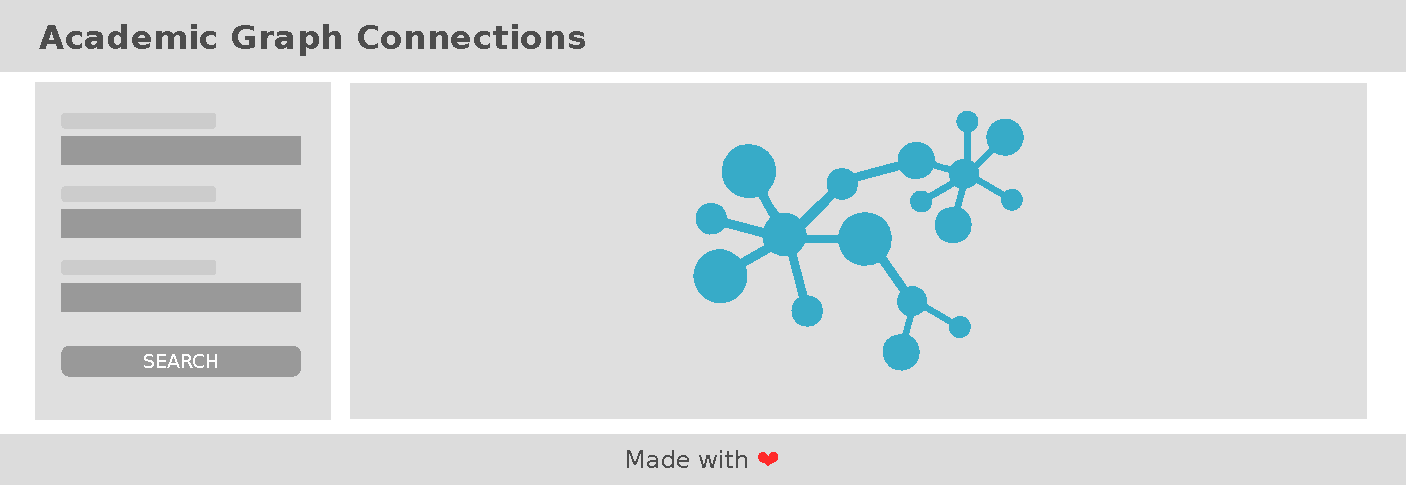
\includegraphics[width=1\textwidth-2pt]{images/chapter4/frontendlayout.pdf}%
	\caption[Layout of the frontend interface with bootstrap]{Layout of the frontend interface with \Gls{bootstrap}: Header row, Content row made of Search Form column component and the Graph column component, Footer row}%
	\label{fig:frontendlayout}
\end{figure}%

By making use of \texttt{\Gls{bootstrap}} for React, \texttt{Header}, \texttt{Content}, \texttt{Footer} are defined and the \texttt{Content} is divided into two columns:
\setlist{nolistsep} \begin{itemize}[noitemsep]
	\item one that will host the search form component,
	\item and the other - the area where the graph is going to be displayed;
\end{itemize}
as shown in \hyperref[fig:frontendlayout]{\autoref{fig:frontendlayout}}.
The ratios of the columns are about 1/4 for the search form and 3/4 for the graph area.

Having created the basis of the website with the placeholders for the components, it is time to present the development of the Search Form component.

\subsection{Search Form component} \label{subsection:ImplementingtheWebApp/Thefrontend/SearchFormcomponent}
In explaining the implementation of the \gls{GraphQL} API in \hyperref[subsubsection:ImplementingtheWebApp/TheAPI/Resolvers/AutocompletesuggestionqueryforstringtoIDtranslation]{\S\ \ref{subsubsection:ImplementingtheWebApp/TheAPI/Resolvers/AutocompletesuggestionqueryforstringtoIDtranslation}} on \hyperref[tobementionedthefrontendthreeinputs]{page \pageref*{tobementionedthefrontendthreeinputs}} is briefly mentioned that the user will have to insert three values in order to perform a search and thus request the collaboration graph of an entity.
These values are:
\setlist{nolistsep} \begin{itemize}[noitemsep]
	\item a string text referred to the name or the title of the start node, the focal entity of the graph around which the collaboration community is built.
	\item the number of minimum depth/hops, that is the number of edge traversals from the start node and further - distant nodes to include in the graph.
	\item the number of maximum depth/hops, that is the number of edge traversals from the start node and nearer - distant nodes to include in the graph. The intersection of min and max depth makes it possible to include in the graph only the nodes belonging to that intersection.
\end{itemize}

For each of these three values there is a distinct form field to be filled.
In the following paragraphs each of these fields is explained in detail.

\begin{figure}[H]%
	\centering%
	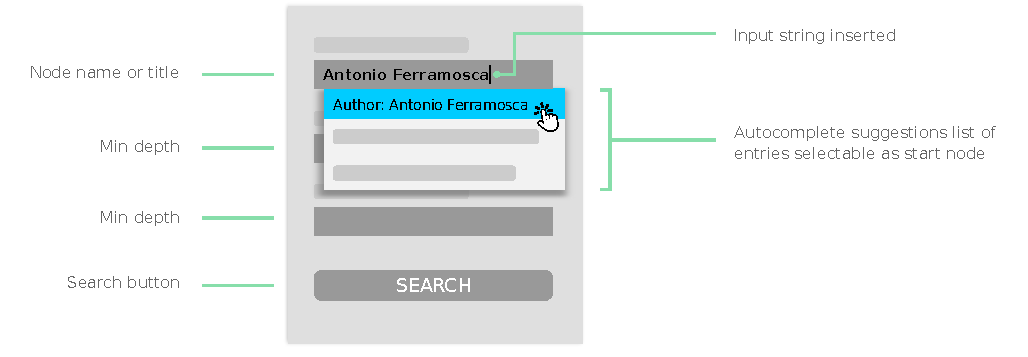
\includegraphics[width=1\textwidth]{images/chapter4/frontendsearchformautocomplete.pdf}%
	\caption[Search Form with autocomplete suggestions: search string "Antonio Ferramosca"]{Search Form with autocomplete suggestions: search string "Antonio Ferramosca"}%
	\label{fig:frontendsearchformautocomplete}
\end{figure}%

\subsubsection{Start vertex}\label{subsubsection:ImplementingtheWebApp/Thefrontend/SearchFormcomponent/Startvertex}
Previously, presenting the implementation of the \acrshort{API}, were mentioned the reasons why there is a need to translate the input string to an id.
See \hyperref[subsubsection:ImplementingtheWebApp/TheAPI/Resolvers/AutocompletesuggestionqueryforstringtoIDtranslation]{\S\ \ref{subsubsection:ImplementingtheWebApp/TheAPI/Resolvers/AutocompletesuggestionqueryforstringtoIDtranslation}} on \hyperref[tobementionedthefrontendtranslationnametoid]{page \pageref*{tobementionedthefrontendtranslationnametoid}}.

The start vertex can be an author e.g.: "Antonio Ferramosca" (as shown in \hyperref[fig:frontendsearchformautocomplete]{\autoref{fig:frontendsearchformautocomplete}}) or an institution e.g.: "University of Bergamo" or whatever vertex type like title of a publication, publisher, journal, editor, series, institution etc. .
To obtain the mapping of the input string from a humanly meaningful string to an id, an autocomplete suggestion feature is implemented.
The user inputs the intended string representing the name or title of the vertex.
That string is sent to the \gls{backend} \acrshort{API}, which performs a request to the database with a filter of all the nodes named that way.
In \hyperref[code:adomainthatrocksfrontend/SearchFormNodeGraph]{\autoref{code:adomainthatrocksfrontend/SearchFormNodeGraph}} is shown the \gls{GraphQL} query the frontend's Search Form Component builds and sends to the backend \acrshort{API}.

\noindent\begin{minipage}{\linewidth} % Wraps the lstlisting inside a minipage of width \linewidth with no indentation to prevent it from splitting between pages
    \lstinputlisting[% will split at page breaks
    	linerange = {103-113},% choose line numbers to include
    	firstnumber = 103,%
    	language = TypeScript,
    	mathescape = false,
    	label = {code:adomainthatrocksfrontend/SearchFormNodeGraph},
    	caption = {[GraphQL query in Search Form component for autocomplete suggestions]\gls{GraphQL query} in Search Form component for autocomplete suggestions}
    ]{code/adomainthatrocksfrontend/SearchFormNodeGraph.tsx}
\end{minipage}

Once done, a list of possible vertices is brought back to the frontend and shown as a suggestion list. The list is a dictionary of the name of the vertex and its id.
For the visual result, see \hyperref[fig:SnapshotSearchFormGargantini]{\autoref{fig:SnapshotSearchFormGargantini}} in \hyperref[section:Displayoftheresults/Frontendsearchform]{\S\ \ref{section:Displayoftheresults/Frontendsearchform} - \nameref{section:Displayoftheresults/Frontendsearchform}}, \hyperref[fig:SnapshotSearchFormGargantini]{page \pageref{fig:SnapshotSearchFormGargantini}}.
The user selects an item from the list and that gets saved as an id the state of the search form.

\subsubsection{Hops, minimum and maximum depth}\label{subsubsection:ImplementingtheWebApp/Thefrontend/SearchFormcomponent/Hopsminimumandmaximumdepth}
The hops range is inserted as minimum and maximum depth of traversal.
The default minimum depth is set to 1 and maximum depth is set to 2.
A minimum and maximum depth of both selected as 1 requests all vertices directly connected to the start vertex.
Whereas a minimum and maximum depth of both selected as 2 requests all vertices that are exactly at 2 hops distance from the start vertex.
In the results of this search would not be present the vertices directly connected to the start vertex.
If the minimum depth is set to 1 and the maximum to 2, then both the 1 hop and 2 hops distant vertices would be included in the results.
The same logic follows for higher minimum and maximum depth values.

\begin{figure}[H]%
	\centering%
	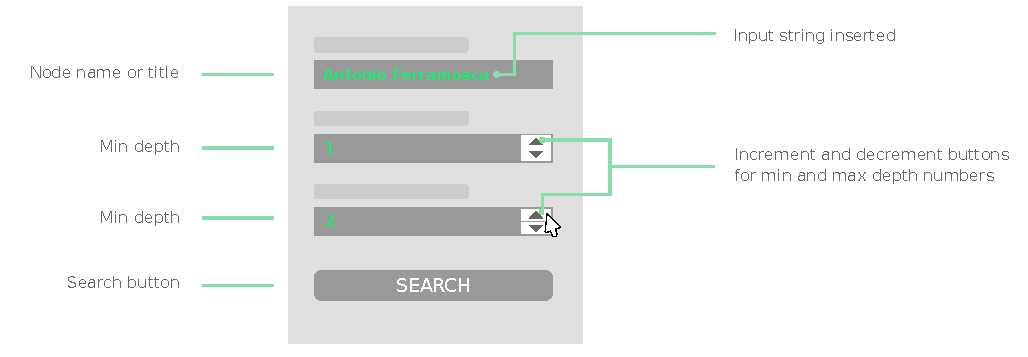
\includegraphics[width=1\textwidth]{images/chapter4/frontendsearchminmaxdepth.pdf}%
	\caption[Search Form's min and max depth values]{Search Form's min and max depth values}%
	\label{fig:frontendsearchminmaxdepth}
\end{figure}%

\medskip

\begin{remark}[on big depth values]\label{remark:onbigdepthvalues}
	Should be noted that a maximum depth of 3 produces a graph of about 250 thousand vertices.
    Users client machine might not be able to render or fit a graph with that many nodes.
    A maximum depth of 4 produces a graph with about 1 million nodes. It takes about 30 seconds for ArangoDB to perform that traversal.
    A maximum depth of 5 produces a graph with many million nodes. For ArangoDB it takes from 15 minutes to an hour to perform that traversal.
    It produces a response a few hundreds of MB total size, if not some GB. The WebApp is not designed to handle these cases. This situation is indicated as in need of a possible improvement in \hyperref[chapter:Conclusions]{\textnormal{\S\ \ref{chapter:Conclusions} - \nameref{chapter:Conclusions}}} \adforn{43}\  \hyperref[section:Conclusions/Possibleimprovements]{\textnormal{\S\ \ref{section:Conclusions/Possibleimprovements} - \nameref{section:Conclusions/Possibleimprovements}}}, specifically in \hyperref[subsection:Conclusions/Possibleimprovements/Limitmaximumnumberofnodesinthefrontendgraph]{\textnormal{\S\ \ref{subsection:Conclusions/Possibleimprovements/Limitmaximumnumberofnodesinthefrontendgraph} - \nameref{subsection:Conclusions/Possibleimprovements/Limitmaximumnumberofnodesinthefrontendgraph}}}, on \hyperref[subsection:Conclusions/Possibleimprovements/Limitmaximumnumberofnodesinthefrontendgraph]{page \pageref{subsection:Conclusions/Possibleimprovements/Limitmaximumnumberofnodesinthefrontendgraph}}.
    Imposing a limit on the maximum number of nodes to obtain, some kind of an upper bound, would be a trade-off between completeness and usability but might still be a reasonable improvement in order to cover also the display of graphs with high values of depths.
\end{remark}

\subsubsection{Search inputs validation}\label{subsection:ImplementingtheWebApp/Thefrontend/SearchFormcomponent/Searchinputsvalidation}
The inputs are validated client side with some basic rules.
If an item from the suggestion list is not selected, thus no id is indicated, the form is considered invalid - warnings in red are shown to the user.

If the minimum depth is not 1 or greater, the form is invalid.
If the maximum depth is not greater or equal to the minimum depth, the form is invalid.
In all other cases the search request for the graph gets sent to the \gls{backend}, provided that an element is already selected from the autocomplete of the name/title.
If the form is valid borders of the fields are colored in green.

\begin{remark}[on server side validation]\label{remark:onserversidevalidation}
	Should be noted that unvalidated queries from the frontend can be sent to the \acrshort{API} through other clients and no check is performed in the backend.
	For example in the case of very big values of depths, the database received the query and tries to do its best to compute a result and return it.
	But sometimes, especially when the query computation overloads the DB host machine, this leads to an automatic interruption of the connection between the \acrshort{API} and the ArangoDB DBMS and the cancellation of all ongoing query computations. 
	
	It is outside the goals of this work to implement security features, thus server side validation was neglected.
\end{remark}
\medskip

Having described the features of the search form, it is time to present the graph rendering component that would display the collaboration networks.
Before that, how the collaboration graph data get requested is presented.

\subsection{Requesting collaboration graph data} \label{subsection:ImplementingtheWebApp/Thefrontend/Requestingcollaborationgraphdata/}
In a similar fashion to how the \gls{GraphQL} \acrshort{API} was queried for vertex suggestions, is queries also for the collaboration graph data.
The only change is that now the response data shall contain types of elements that are not anymore that simple or primitive.

When querying about suggestions, the response was an array of strings.
While for graph data the response shall be composed of arrays of objects having diffrent attributes.
To this end, \gls{GraphQL} comes to help with its type system.
In \hyperref[code:adomainthatrocksfrontend/Content]{\autoref{code:adomainthatrocksfrontend/Content}}, lines 22-24 inline fragments (spread operator) are (is) used to access data on the underlying concrete type.

\noindent\lstinputlisting[% will split at page breaks
	linerange = {16-29},% choose line numbers to include
	firstnumber = 16,%
	language = TypeScript,
	mathescape = false,
	label = {code:adomainthatrocksfrontend/Content},
	caption = {[GraphQL query to request graph data from the API]\gls{GraphQL query} to request graph data from the \acrshort{API}}
]{code/adomainthatrocksfrontend/Content.tsx}
\medskip

With the graph data obtained from the backend, it is now possible to start drawing graphs in the dedicated area.
In the following subsection the graph rendering component's features are brought.

\subsection{Graph rendering component} \label{subsection:ImplementingtheWebApp/Thefrontend/Graphrenderingcomponent}
There exist many different JavaScript graph visualization libraries with different features.
To show a network graph with simple and compound nodes (used for communities), \gls{Cytoscape.JS} \texttt{\gls{Cytoscape}} was deemed appropriate.
\medskip

\gls{Cytoscape.JS} is an open-source graph theory library written in JavaScript.
It makes developer's life easier for displaying and manipulating rich, interactive graphs.

\gls{Cytoscape} is domain independent but usually when used by social scientists, it is employed to visualize and analyze large social networks of interpersonal relationships.
It has many extensions and is able to perform analytical computations.
It even provides different clustering algorithms, such as the ones shown in \hyperref[longtable:cytoscapeclusteringalgorithms]{\autoref{longtable:cytoscapeclusteringalgorithms}}

\begin{center}
	\vspace*{-0.25cm}
	\begin{longtable}{p{0.47\linewidth}p{0.47\linewidth}}
		\hline \hline
		\textbf{Attribute Cluster Algorithms} & \textbf{Network Cluster Algorithms}\\
		\hline \hline
		\endfirsthead
		
		\multicolumn{2}{l}{... continued from previous page}\\
		\hline \hline
		\textbf{Attribute Cluster Algorithms} & \textbf{Network Cluster Algorithms}\\
		\hline \hline
		\endhead
		
		\hline
		\caption*{\tablename\ \thetable{}: \nameref*{longtable:cytoscapeclusteringalgorithms}. Continues on next page ...}
		\vspace*{0.5cm}
		\endfoot
		
		\hline
		%\multicolumn{2}{| c |}{End of Table}\\
		%\hline
		\caption[Clustering algorithms provided by Cytoscape]{Clustering algorithms provided by \gls{Cytoscape}}\label{longtable:cytoscapeclusteringalgorithms}
		\vspace*{0.5cm}
		\endlastfoot

        & --\ Affinity Propagation\\
        --\ AutoSOME Clustering & --\ Connected Components\\
        --\ Creating Correlation Networks & --\ Community Clustering (GLay)\\
        --\ Hierarchical Clustering & --\ MCODE\\
        --\ K-Means Clustering & --\ MCL\\
        --\ K-Medoid Clustering & --\ SCPS (Spectral Clustering of Protein Sequences)\\
        & --\ Transitivity Clustering\\
		\hline
	\end{longtable}
	\vspace*{-1.35cm}
\end{center}

\gls{Cytoscape.JS} includes all the gestures expected out-of-the-box, such as pinch-to-zoom, box selection, panning, etc.\sfcite{CytoscapeJS2021, PlotlyReactCytoscapeJS2021}

In order to render a graph, it needs just - as one would expect - a set of vertices and a set of edges.
More details follow in the next subsubsections.

\subsection{Sets of vertices and edges} \label{subsection:ImplementingtheWebApp/Thefrontend/Graphrenderingcomponent/Setsofverticesandedges}
\begin{sublstlisting}
    \noindent\begin{minipage}{\linewidth} % Wraps the lstlisting inside a minipage of width \linewidth with no indentation to prevent it from splitting between pages
        \lstinputlisting[
            %nolol, % will not appear in list of code listings
            linerange = {107-112}, % choose line numbers to include
            firstnumber = 107,
            language = TypeScript,
            mathescape = false,
            label = {code:adomainthatrocksfrontend/CytoscapeGraph107},
            caption = {[\ \ \ \ \ \ \ Vertices with community stated as parent node]Vertices with community stated as parent node}
        ]{code/adomainthatrocksfrontend/CytoscapeGraph.tsx}
    \end{minipage}
    
    With \gls{Cytoscape}, a vertex in the set of vertices has to have an \texttt{id} property and a \texttt{label}.
    The \texttt{id} must be distinct.
    If it belongs to or is inside a compound node as shown in \hyperref[code:adomainthatrocksfrontend/CytoscapeGraph107]{\autoref{code:adomainthatrocksfrontend/CytoscapeGraph107}} it also has a parent attribute.
    For each node, styling of the shape, size and color or text format - is applicable.
    On vertex click, vertex information is shown in a pop-up.
    \medskip

    An edge on the other hand has a \texttt{source}, a \texttt{target} and a \texttt{label} attribute as shown in \hyperref[code:adomainthatrocksfrontend/CytoscapeGraph137]{\autoref{code:adomainthatrocksfrontend/CytoscapeGraph137}}.
    The \texttt{source} and \texttt{target} values have to be \texttt{id}s present in the set of vertices.
    Edges too can be styled with properties like color, thickness etc.
    
    \noindent\begin{minipage}{\linewidth} % Wraps the lstlisting inside a minipage of width \linewidth with no indentation to prevent it from splitting between pages
        \lstinputlisting[
            %nolol, % will not appear in list of code listings
            linerange = {137-142}, % choose line numbers to include
            firstnumber = 137,
            language = TypeScript,
            mathescape = false,
            label = {code:adomainthatrocksfrontend/CytoscapeGraph137},
            caption = {[\ \ \ \ \ \ \ Edges with source and target vertices]Edges with source and target vertices}
        ]{code/adomainthatrocksfrontend/CytoscapeGraph.tsx}
    \end{minipage}
    
    \subsection{Sets of communities and compound nodes} \label{subsection:ImplementingtheWebApp/Thefrontend/Graphrenderingcomponent/Setsofcommunitiesandcompoundnodes}
    Using the \texttt{CoseBilken} layout of \gls{Cytoscape.JS}, it is possible to properly fit and render compound nodes, that is the community nodes acting as parents for the vertices that belong to them.
    Compound nodes have as their properties an \texttt{id} and a \texttt{label} as shown in \hyperref[code:adomainthatrocksfrontend/CytoscapeGraph149]{\autoref{code:adomainthatrocksfrontend/CytoscapeGraph149}}.
    The \texttt{id} must be distinct between all nodes.
    Since the same community generally appears many times (as parent of different vertices) in a collaboration graph, it may happen that the communities the API provides are included multiple times in the response, as many as the number of vertices belonging to that community.
    This generates errors with \gls{Cytoscape.JS} (\texttt{id}s must be unique) and is avoided by changing the APIs AQL query to the database in order to request a list of distinct communities.
    \medskip

    \noindent\begin{minipage}{\linewidth} % Wraps the lstlisting inside a minipage of width \linewidth with no indentation to prevent it from splitting between pages
        \noindent\lstinputlisting[
            %nolol, % will not appear in list of code listings
            linerange = {149-153}, % choose line numbers to include
            firstnumber = 149,
            language = TypeScript,
            mathescape = false,
            label = {code:adomainthatrocksfrontend/CytoscapeGraph149},
            caption = {[\ \ \ \ \ \ \ Communities, the compound nodes]Communities, the compound nodes}
        ]{code/adomainthatrocksfrontend/CytoscapeGraph.tsx}
    \end{minipage}%
    
    In the end, all elements of the collaboration graph are feeded together to \gls{Cytoscape} like in \hyperref[code:adomainthatrocksfrontend/CytoscapeGraph166]{\autoref{code:adomainthatrocksfrontend/CytoscapeGraph166}} and the library handles the positioning of the elements in the drawing area.
    Initially set to random positions, using gravity and repelling forces between the elements, it is possible to fit them all in a nice graph.

    \noindent\begin{minipage}{\linewidth} % Wraps the lstlisting inside a minipage of width \linewidth with no indentation to prevent it from splitting between pages
        \noindent\lstinputlisting[
            %nolol, % will not appear in list of code listings
            linerange = {166-168}, % choose line numbers to include
            firstnumber = 166,
            language = TypeScript,
            mathescape = false,
            label = {code:adomainthatrocksfrontend/CytoscapeGraph166},
            caption = {[\ \ \ \ \ \ \ All graph elements joined using spread operator expansion]All graph elements joined using spread operator expansion}
        ]{code/adomainthatrocksfrontend/CytoscapeGraph.tsx}
    \end{minipage}%
\end{sublstlisting}%
\setcounter{lstlisting}{\value{parentlstlisting}-1}%
\vspace*{-5.7pt}%
\begin{lstlisting}[%
    label = {code:adomainthatrocksfrontend/CytoscapeGraph},%
    caption = {[\ Cytoscape Graph Component source code snippets for the definition of the constituting elements of the col\-la\-bo\-ra\-tion graph]\gls{Cytoscape} Graph Component source code snippets for the definition of the constituting elements of the collaboration graph},%
    framesep=0pt,%
    framerule=0pt,%
    frame={tb}%
]
\end{lstlisting}

Having seen the community detection algorithm execution and now the implementation of the Web App, in the next chapter are going to be presented some concrete views of different collaboration graphs visualized in the Web App's frontend UI.
\newpage
\thispagestyle{empty}
